% Copyright (C) 2018 Liu Yifan, Zhao Tianyu 
% Permission is granted to copy, distribute and/or modify this document
% under the terms of the GNU Free Documentation License, Version 1.3
% or any later version published by the Free Software Foundation;
% with no Invariant Sections, no FrontCover Texts, and no BackCover Texts.
% A copy of the license is included in the section entitled "GNU
% Free Documentation License".
%%%%%%%%%%%%%%%%重要的事情现在前面,第一次编译点左上角选 Compiler(编译器)为XeLaTeX%%%%%%%%%%%%
\documentclass[zihao=-4,a4paper]{ctexart}

% 论文基本配置,加载宏包、数学命令等全局配置
% Copyright (C) 2018 Liu Yifan, Zhao Tianyu 
% Permission is granted to copy, distribute and/or modify this document
% under the terms of the GNU Free Documentation License, Version 1.3
% or any later version published by the Free Software Foundation;
% with no Invariant Sections, no FrontCover Texts, and no BackCover Texts.
% A copy of the license is included in the section entitled "GNU
% Free Documentation License".
\usepackage{ctex}
\setCJKmainfont[AutoFakeBold=2, ItalicFont={simsun.ttc}]{simsun.ttc}
\setmainfont{Times New Roman} 
\usepackage{fontspec}
\usepackage{amsmath}
\usepackage{amssymb}
\usepackage{hyperref} 
\usepackage{amsthm} 
\usepackage{mathtools} 
\usepackage{mathrsfs}
\usepackage{fancyhdr}
\usepackage{enumerate}
\usepackage{metalogo}
% \usepackage{mathscr}
\numberwithin{equation}{section}
\newtheorem{definition}{定义}[section]
\newtheorem{example}{例}[section]
\newtheorem{theorem}{定理}[section]
\newtheorem*{maintheorem}{主要定理}
\newtheorem{question}{问题}
\newtheorem{lemma}[theorem]{引理}
\newtheorem{remark}[theorem]{备注}
\newtheorem{corollary}[theorem]{推论}
\newtheorem{proposition}[theorem]{命题}
%\songti
% \newtheorem{algorithm}
\ctexset{section={format={\zihao{3}\bfseries},
			name = {第,章},beforeskip=0.5ex plus 20pt,afterskip=10pt}}
\ctexset{subsection={format={\zihao{4}\bfseries },
				beforeskip=0.75ex,afterskip=0.95ex}}
\ctexset{subsubsection={format={\zihao{-4}\bfseries },
				beforeskip=0.75ex,afterskip=0.95ex}}

\usepackage[labelfont=bf]{caption}
\captionsetup{font={small},labelsep=space}
\numberwithin{figure}{section}
\renewcommand{\proofname}{\zihao{-4}  \bfseries 证明}
\usepackage{geometry}
\geometry{top=2.5cm,bottom=2.5cm,left=3cm,right=2.5cm,headsep=0.5cm}
%\setmainfont{Times New Roman}
\ctexset{abstractname={\zihao{3}   摘\hspace*{2em} 要}}
%\ctexset{abstract={beforskip={20pt}
  %                 afterskip=10pt}}
%\ctexset{section ={name = {第,章},beforeskip=20pt,afterskip=10pt}}		     
\ctexset{bibname={\centerline{ \zihao{3}  参\hspace*{0.5em}考\hspace*{0.5em}文\hspace*{0.5em}献}}}

\usepackage{setspace}

\usepackage{cite}
\usepackage{listings} 
\usepackage[sort]{natbib}
\setcitestyle{numbers,square,comma}
%\setlength{\bibspacing}{\baselineskip}

\newcommand{\upcite}[1]{\textsuperscript{\cite{#1}}}

\makeatletter
\def\@cite#1#2{\textsuperscript{[{#1\if@tempswa , #2\fi}]}}
\makeatother

\usepackage{titletoc}
\titlecontents{section}[0pt]{\addvspace{2pt}\filright}
{\contentspush{\thecontentslabel\ }}
{}{\titlerule*[8pt]{.}\contentspage}
%%%%commented%%%%
%\usepackage{enumitem}
%\setenumerate{fullwidth,itemindent=\parindent,listparindent=\parindent,itemsep=0ex,partopsep=0pt,parsep=0ex}

\usepackage{graphicx}
\usepackage{caption}
\usepackage{subfigure}
%%%%%%%%%%%%%5
\usepackage{enumerate}
\usepackage{minted}
%%%%%%%%%%%%%
\usepackage{pdfpages}
\usepackage{afterpage}
\allowdisplaybreaks[1]


\newcommand{\h}{\tilde{h}}
\renewcommand{\k}{\kappa}
\renewcommand{\b}{\beta}
\renewcommand{\t}{\theta}
\newcommand{\la}{\lambda}
\newcommand{\La}{\Lambda}
\newcommand{\kk}{\tilde{\kappa}}
\renewcommand{\L}{\mathscr{L}}
\newcommand{\A}{\mathscr{A}}
\newcommand{\F}{\mathbf{F}}
\newcommand{\p}{\mathbf{p}}
%%%%%%%%%%%%%%%%%fanfan%%%%%%

\newcommand{\blank}[1]{\hspace*{#1}}
\newcommand{\sectionend}{\ifodd\value{page}\afterpage{\null}\else\fi\newpage\vspace*{0pt}}
\usepackage{dutchcal}
%%%%%%%%%%%%%%%%%%%%%%%%%%%%%%%

\pagestyle{fancy}
\lhead{}
\rhead{}
\chead{\zihao{-5} 无人驾驶车辆路径规划与车道保持强化学习方法}
\cfoot{\zihao{-5} \thepage}
\renewcommand{\headrulewidth}{0.4pt}
\renewcommand{\footrulewidth}{0pt}



\title{\zihao{2} \bfseries  无人驾驶车辆路径规划与车道保持强化学习方法}
\author{}
\date{}



% 表格中支持跨行
%\usepackage{multirow}

% 跨页表格
%\usepackage{longtable}

% 固定宽度的表格
%\usepackage{tabularx}

% 表格中的反斜线
%\usepackage{diagbox}

% 确定浮动对象的位置,可以使用 H,强制将浮动对象放到这里(可能效果很差)
%\usepackage{float}

% 浮动图形控制宏包。
% 允许上一个 section 的浮动图形出现在下一个 section 的开始部分
% 该宏包提供处理浮动对象的 \FloatBarrier 命令,使所有未处
% 理的浮动图形立即被处理。这三个宏包仅供参考,未必使用:
% \usepackage[below]{placeins}
% \usepackage{floatflt} % 图文混排用宏包
% \usepackage{rotating} % 图形和表格的控制旋转

% 定理类环境宏包
%\usepackage[amsmath,thmmarks,hyperref]{ntheorem}


% 数学命令
%% Adapted for use with thuthesis.
% Original code is at https://github.com/goodfeli/dlbook_notation/blob/master/math_commands.tex

%%%%% NEW MATH DEFINITIONS %%%%%

\newcommand\ceil[1]{\lceil #1 \rceil}
\newcommand\floor[1]{\lfloor #1 \rfloor}


% Vectors
\newcommand\Vector[1]{\symbf{#1}}

\newcommand\0{{\Vector{0}}}
\newcommand\vzero{{\Vector{0}}}
\newcommand\1{{\Vector{1}}}
\newcommand\vone{{\Vector{1}}}

\newcommand\va{{\Vector{a}}}
\newcommand\vb{{\Vector{b}}}
\newcommand\vc{{\Vector{c}}}
\newcommand\vd{{\Vector{d}}}
\newcommand\ve{{\Vector{e}}}
\newcommand\vf{{\Vector{f}}}
\newcommand\vg{{\Vector{g}}}
\newcommand\vh{{\Vector{h}}}
\newcommand\vi{{\Vector{i}}}
\newcommand\vj{{\Vector{j}}}
\newcommand\vk{{\Vector{k}}}
\newcommand\vl{{\Vector{l}}}
\newcommand\vm{{\Vector{m}}}
\newcommand\vn{{\Vector{n}}}
\newcommand\vo{{\Vector{o}}}
\newcommand\vp{{\Vector{p}}}
\newcommand\vq{{\Vector{q}}}
\newcommand\vr{{\Vector{r}}}
\newcommand\vs{{\Vector{s}}}
\newcommand\vt{{\Vector{t}}}
\newcommand\vu{{\Vector{u}}}
\newcommand\vv{{\Vector{v}}}
\newcommand\vw{{\Vector{w}}}
\newcommand\vx{{\Vector{x}}}
\newcommand\vy{{\Vector{y}}}
\newcommand\vz{{\Vector{z}}}

\newcommand\valpha{{\Vector{\alpha}}}
\newcommand\vbeta{{\Vector{\beta}}}
\newcommand\vgamma{{\Vector{\gamma}}}
\newcommand\vdelta{{\Vector{\delta}}}
\newcommand\vepsilon{{\Vector{\epsilon}}}
\newcommand\vtheta{{\Vector{\theta}}}
\newcommand\viota{{\Vector{\iota}}}
\newcommand\vkappa{{\Vector{\kappa}}}
\newcommand\vlambda{{\Vector{\lambda}}}
\newcommand\vmu{{\Vector{\mu}}}
\newcommand\vnu{{\Vector{\nu}}}
\newcommand\vxi{{\Vector{\xi}}}
\newcommand\vpi{{\Vector{\pi}}}
\newcommand\vrho{{\Vector{\rho}}}
\newcommand\vsigma{{\Vector{\sigma}}}
\newcommand\vtau{{\Vector{\tau}}}
\newcommand\vupsilon{{\Vector{\upsilon}}}
\newcommand\vphi{{\Vector{\phi}}}
\newcommand\vchi{{\Vector{\chi}}}
\newcommand\vpsi{{\Vector{\psi}}}
\newcommand\vomega{{\Vector{\omega}}}


% Matrix
\newcommand\MATRIX[1]{\symbf{#1}}

\newcommand\mA{{\MATRIX{A}}}
\newcommand\mB{{\MATRIX{B}}}
\newcommand\mC{{\MATRIX{C}}}
\newcommand\mD{{\MATRIX{D}}}
\newcommand\mE{{\MATRIX{E}}}
\newcommand\mF{{\MATRIX{F}}}
\newcommand\mG{{\MATRIX{G}}}
\newcommand\mH{{\MATRIX{H}}}
\newcommand\mI{{\MATRIX{I}}}
\newcommand\mJ{{\MATRIX{J}}}
\newcommand\mK{{\MATRIX{K}}}
\newcommand\mL{{\MATRIX{L}}}
\newcommand\mM{{\MATRIX{M}}}
\newcommand\mN{{\MATRIX{N}}}
\newcommand\mO{{\MATRIX{O}}}
\newcommand\mP{{\MATRIX{P}}}
\newcommand\mQ{{\MATRIX{Q}}}
\newcommand\mR{{\MATRIX{R}}}
\newcommand\mS{{\MATRIX{S}}}
\newcommand\mT{{\MATRIX{T}}}
\newcommand\mU{{\MATRIX{U}}}
\newcommand\mV{{\MATRIX{V}}}
\newcommand\mW{{\MATRIX{W}}}
\newcommand\mX{{\MATRIX{X}}}
\newcommand\mY{{\MATRIX{Y}}}
\newcommand\mZ{{\MATRIX{Z}}}

\newcommand\mGamma{{\MATRIX{\Gamma}}}
\newcommand\mDelta{{\MATRIX{\Delta}}}
\newcommand\mTheta{{\MATRIX{\Theta}}}
\newcommand\mLambda{{\MATRIX{\Lambda}}}
\newcommand\mXi{{\MATRIX{\Xi}}}
\newcommand\mPi{{\MATRIX{\Pi}}}
\newcommand\mSigma{{\MATRIX{\Sigma}}}
\newcommand\mUpsilon{{\MATRIX{\Upsilon}}}
\newcommand\mPhi{{\MATRIX{\Phi}}}
\newcommand\mPsi{{\MATRIX{\Psi}}}
\newcommand\mOmega{{\MATRIX{\Omega}}}


% Tensor
\newcommand\tens[1]{\symbfsf{#1}}
\newcommand\tA{{\tens{A}}}
\newcommand\tB{{\tens{B}}}
\newcommand\tC{{\tens{C}}}
\newcommand\tD{{\tens{D}}}
\newcommand\tE{{\tens{E}}}
\newcommand\tF{{\tens{F}}}
\newcommand\tG{{\tens{G}}}
\newcommand\tH{{\tens{H}}}
\newcommand\tI{{\tens{I}}}
\newcommand\tJ{{\tens{J}}}
\newcommand\tK{{\tens{K}}}
\newcommand\tL{{\tens{L}}}
\newcommand\tM{{\tens{M}}}
\newcommand\tN{{\tens{N}}}
\newcommand\tO{{\tens{O}}}
\newcommand\tP{{\tens{P}}}
\newcommand\tQ{{\tens{Q}}}
\newcommand\tR{{\tens{R}}}
\newcommand\tS{{\tens{S}}}
\newcommand\tT{{\tens{T}}}
\newcommand\tU{{\tens{U}}}
\newcommand\tV{{\tens{V}}}
\newcommand\tW{{\tens{W}}}
\newcommand\tX{{\tens{X}}}
\newcommand\tY{{\tens{Y}}}
\newcommand\tZ{{\tens{Z}}}


% Graph
\newcommand\gA{{\mathcal{A}}}
\newcommand\gB{{\mathcal{B}}}
\newcommand\gC{{\mathcal{C}}}
\newcommand\gD{{\mathcal{D}}}
\newcommand\gE{{\mathcal{E}}}
\newcommand\gF{{\mathcal{F}}}
\newcommand\gG{{\mathcal{G}}}
\newcommand\gH{{\mathcal{H}}}
\newcommand\gI{{\mathcal{I}}}
\newcommand\gJ{{\mathcal{J}}}
\newcommand\gK{{\mathcal{K}}}
\newcommand\gL{{\mathcal{L}}}
\newcommand\gM{{\mathcal{M}}}
\newcommand\gN{{\mathcal{N}}}
\newcommand\gO{{\mathcal{O}}}
\newcommand\gP{{\mathcal{P}}}
\newcommand\gQ{{\mathcal{Q}}}
\newcommand\gR{{\mathcal{R}}}
\newcommand\gS{{\mathcal{S}}}
\newcommand\gT{{\mathcal{T}}}
\newcommand\gU{{\mathcal{U}}}
\newcommand\gV{{\mathcal{V}}}
\newcommand\gW{{\mathcal{W}}}
\newcommand\gX{{\mathcal{X}}}
\newcommand\gY{{\mathcal{Y}}}
\newcommand\gZ{{\mathcal{Z}}}


% Sets
\newcommand\sA{{\mathbb{A}}}
\newcommand\sB{{\mathbb{B}}}
\newcommand\sC{{\mathbb{C}}}
\newcommand\sD{{\mathbb{D}}}
% Don't use a set called E, because this would be the same as our symbol
% for expectation.
\newcommand\sF{{\mathbb{F}}}
\newcommand\sG{{\mathbb{G}}}
\newcommand\sH{{\mathbb{H}}}
\newcommand\sI{{\mathbb{I}}}
\newcommand\sJ{{\mathbb{J}}}
\newcommand\sK{{\mathbb{K}}}
\newcommand\sL{{\mathbb{L}}}
\newcommand\sM{{\mathbb{M}}}
\newcommand\sN{{\mathbb{N}}}
\newcommand\sO{{\mathbb{O}}}
\newcommand\sP{{\mathbb{P}}}
\newcommand\sQ{{\mathbb{Q}}}
\newcommand\sR{{\mathbb{R}}}
\newcommand\sS{{\mathbb{S}}}
\newcommand\sT{{\mathbb{T}}}
\newcommand\sU{{\mathbb{U}}}
\newcommand\sV{{\mathbb{V}}}
\newcommand\sW{{\mathbb{W}}}
\newcommand\sX{{\mathbb{X}}}
\newcommand\sY{{\mathbb{Y}}}
\newcommand\sZ{{\mathbb{Z}}}


% Random variables
\newcommand\RandomVariable[1]{\symit{#1}}

\newcommand\rA{{\RandomVariable{A}}}
\newcommand\rB{{\RandomVariable{B}}}
\newcommand\rC{{\RandomVariable{C}}}
\newcommand\rD{{\RandomVariable{D}}}
\newcommand\rE{{\RandomVariable{E}}}
\newcommand\rF{{\RandomVariable{F}}}
\newcommand\rG{{\RandomVariable{G}}}
\newcommand\rH{{\RandomVariable{H}}}
\newcommand\rI{{\RandomVariable{I}}}
\newcommand\rJ{{\RandomVariable{J}}}
\newcommand\rK{{\RandomVariable{K}}}
\newcommand\rL{{\RandomVariable{L}}}
\newcommand\rM{{\RandomVariable{M}}}
\newcommand\rN{{\RandomVariable{N}}}
\newcommand\rO{{\RandomVariable{O}}}
\newcommand\rP{{\RandomVariable{P}}}
\newcommand\rQ{{\RandomVariable{Q}}}
\newcommand\rR{{\RandomVariable{R}}}
\newcommand\rS{{\RandomVariable{S}}}
\newcommand\rT{{\RandomVariable{T}}}
\newcommand\rU{{\RandomVariable{U}}}
\newcommand\rV{{\RandomVariable{V}}}
\newcommand\rW{{\RandomVariable{W}}}
\newcommand\rX{{\RandomVariable{X}}}
\newcommand\rY{{\RandomVariable{Y}}}
\newcommand\rZ{{\RandomVariable{Z}}}

% Random vectors
\newcommand\RandomVector[1]{\symbf{#1}}

\newcommand\rvA{{\RandomVector{A}}}
\newcommand\rvB{{\RandomVector{B}}}
\newcommand\rvC{{\RandomVector{C}}}
\newcommand\rvD{{\RandomVector{D}}}
\newcommand\rvE{{\RandomVector{E}}}
\newcommand\rvF{{\RandomVector{F}}}
\newcommand\rvG{{\RandomVector{G}}}
\newcommand\rvH{{\RandomVector{H}}}
\newcommand\rvI{{\RandomVector{I}}}
\newcommand\rvJ{{\RandomVector{J}}}
\newcommand\rvK{{\RandomVector{K}}}
\newcommand\rvL{{\RandomVector{L}}}
\newcommand\rvM{{\RandomVector{M}}}
\newcommand\rvN{{\RandomVector{N}}}
\newcommand\rvO{{\RandomVector{O}}}
\newcommand\rvP{{\RandomVector{P}}}
\newcommand\rvQ{{\RandomVector{Q}}}
\newcommand\rvR{{\RandomVector{R}}}
\newcommand\rvS{{\RandomVector{S}}}
\newcommand\rvT{{\RandomVector{T}}}
\newcommand\rvU{{\RandomVector{U}}}
\newcommand\rvV{{\RandomVector{V}}}
\newcommand\rvW{{\RandomVector{W}}}
\newcommand\rvX{{\RandomVector{X}}}
\newcommand\rvY{{\RandomVector{Y}}}
\newcommand\rvZ{{\RandomVector{Z}}}

\newcommand\laplace{\mathrm{Laplace}} % Laplace distribution

\newcommand\E{\mathbb{E}}
\newcommand\Ls{\mathcal{L}}
\newcommand\R{\mathbb{R}}
\newcommand\emp{\tilde{p}}
\newcommand\lr{\alpha}
\newcommand\reg{\lambda}
\newcommand\rect{\mathrm{rectifier}}
\newcommand\softmax{\mathrm{softmax}}
\newcommand\sigmoid{\sigma}
\newcommand\softplus{\zeta}
\newcommand\KL{D_{\mathrm{KL}}}
\newcommand\Var{\mathrm{Var}}
\newcommand\standarderror{\mathrm{SE}}
\newcommand\Cov{\mathrm{Cov}}
% Wolfram Mathworld says $L^2$ is for function spaces and $\ell^2$ is for vectors
% But then they seem to use $L^2$ for vectors throughout the site, and so does
% wikipedia.
\newcommand\normlzero{L^0}
\newcommand\normlone{L^1}
\newcommand\normltwo{L^2}
\newcommand\normlp{L^p}
\newcommand\normmax{L^\infty}

\DeclareMathOperator*{\argmax}{arg\,max}
\DeclareMathOperator*{\argmin}{arg\,min}

\DeclareMathOperator{\sign}{sign}
\DeclareMathOperator{\Tr}{Tr}
\let\ab\allowbreak


% 定义自己常用的东西
% \def\myname{薛瑞尼}
%------------------------算法(伪代码)的环境设置---------------------------------------------- 
\usepackage{algorithm,algpseudocode,float}
%\usepackage{algorithmic}
\usepackage{lipsum}
%\renewcommand{\algorithmicrequire}{\textbf{input:}}   % Use Input in the format of Algorithm  
%\renewcommand{\algorithmicensure}{\textbf{process:}}    % Use Output in the format of Algorithm
\floatname{algorithm}{算法}  
\renewcommand{\algorithmicrequire}{\textbf{输入:}}  
\renewcommand{\algorithmicensure}{\textbf{过程:}} 
\makeatletter
\newenvironment{breakablealgorithm}
  {% \begin{breakablealgorithm}
   \begin{center}
     \refstepcounter{algorithm}% New algorithm
     \hrule height.8pt depth0pt \kern2pt% \@fs@pre for \@fs@ruled
     \renewcommand{\caption}[2][\relax]{% Make a new \caption
       {\raggedright\textbf{\ALG@name~\thealgorithm} ##2\par}%
       \ifx\relax##1\relax % #1 is \relax
         \addcontentsline{loa}{algorithm}{\protect\numberline{\thealgorithm}##2}%
       \else % #1 is not \relax
         \addcontentsline{loa}{algorithm}{\protect\numberline{\thealgorithm}##1}%
       \fi
       \kern2pt\hrule\kern2pt
     }
  }{% \end{breakablealgorithm}
     \kern2pt\hrule\relax% \@fs@post for \@fs@ruled
   \end{center}
  }
\makeatother
% hyperref 宏包在最后调用
\usepackage{hyperref}
\hypersetup{hidelinks} 
% algorithms
%\usepackage[ruled,vlined]{algorithm2e}
%\renewcommand{\algorithmcfname}{算法}

\usepackage{booktabs}
% \usepackage{xcolor}
% 据说加了一行这个查重就不会乱码了
% \usepackage{ccmap}
\begin{document}
        %  \begin{center}
        %   求解多右端线性方程组的一种改进共轭梯度算法研究\\
        %   %{\bfseries \zihao{2} !如果不多加这一行字复制进Word会乱码,导致不能查重!}
        %  \end{center}

	\includepdfmerge{my_cover2.pdf}
	\thispagestyle{plain}
	\pagenumbering{Roman}
	\linespread{1.35}
	\begin{abstract}
	\zihao{-4}{
	随着无人驾驶技术的发展,各种路径规划与无人驾驶决策算法被相继提出,然而现今的路径规划算法大都无法考虑乘客与驾驶人员的习惯。无人驾驶的决策模块也大都基于规则进行设计,其设计成本高且无法适应复杂环境。
	
	针对上述问题,本文使用强化学习的路径规划方法进行路径规划,强化学习可以通过定制奖励函数,来满足不同人的需求。针对无人驾驶决策模块的问题,本文使用深度强化学习中的深度Q学习(DQN)算法进行车道保持决策,其作为一种端到端的算法可以有效解决上述提到的问题。最后,本文在Python+gym环境下验证了本文使用的强化学习算法,其结果表明使用强化学习做路径规划可以满足不同人员的要求;在Carla仿真平台进行了车道保持任务决策,其结果显示使用深度强化学习进行无人驾驶决策具有一定可行性。
  
	{\bfseries  关键词: 路径规划, 深度强化学习, Carla, 车道保持, 无人驾驶,强化学习} }
	\end{abstract}


	

	
	\newpage
	\thispagestyle{plain}
	\renewcommand\abstractname{ABSTRACT}
	
	\begin{abstract}
	\zihao{-4}{
With the development of driverless technology, various path planning and driverless decision-making algorithms are proposed one after another. However, most of the current path planning algorithms cannot consider the habits of passengers and drivers. Most of the decision-making modules of unmanned driving are also designed based on rules, which are expensive to design and cannot adapt to complex environments.
To in  response to the above problems, this thesis uses the reinforcement learning path planning method for path planning. Reinforcement learning can customize the reward function to meet the needs of different people. Aiming at the problem of the driverless decision-making module, this thesis uses the deep Q-learning (DQN) algorithm in deep reinforcement learning to make lane keeping decision-making. As an end-to-end algorithm, it can effectively solve the above-mentioned problems. Finally, this thesis verifies the reinforcement learning algorithm used in this thesis in the Python+gym environment, and the results show that the use of reinforcement learning for path planning can meet the requirements of different personnel; the lane keeping task decision is made on the Carla simulation platform, and the results show that the depth of use Reinforcement learning has certain feasibility for driverless decision-making.

	{\bf Keywords: 
PathPlanner, DeepReinforcementLearning, Carla, Line Keeping, self-driving car,ReinforcementLearning}     }
	\end{abstract}
	
	\newpage
	\thispagestyle{plain}
	\renewcommand\contentsname{\centerline{\zihao{3}    目\hspace*{2em}录}}

	\tableofcontents
	\thispagestyle{plain}
% 
	
	\newpage
	
	%\maketitle
	\thispagestyle{fancy}
	\vspace*{-20pt}
	\begin{center}
	\zihao{3} \bfseries  无人驾驶车辆路径规划与车道保持强化学习方法
	\vspace*{20pt}
	\end{center}
	
	\pagenumbering{arabic}
	
% \mainmatter
% !TeX root = ../dlmu.tex


\section{绪论}
\subsection{无人驾驶及路径规划相关背景}
随着世界经济的腾飞,机动车数量迅速增长。其不可避免的带来了环境与交通事故,
据统计,交通事故是导致现代人非自然死亡的最主要原因,于是研究人员提出可以使用车辆智能化技术即无人驾驶来解决这些难题。目前,无人驾驶已是各国研究的重点,其在缓解交通拥堵,改善空气质
量,提高出行安全方面有着重大意义。各国目前也在无人驾驶领域,给予了企业很多政策和经济上的便利。

据目前通用的业内标准\upcite{r1},无人驾驶有L0\~{}L5六个级别。如表~\ref{tab:tab1}所示,其中L3以上级别,由驾驶设备观测环境,完成汽车加减速等大部分驾驶动作。无人驾驶每个级别的突破都具有极大难度,尤其是L4到L5。目前各个企业研究的重点也都是在L4范围内的自动驾驶。
\begin{table}[H]
  \centering
  \caption{ \textbf{自动驾驶分级标准\upcite{r1}}}
  \begin{tabular}{lc}
    \toprule
    级别          &       自动化程度                         \\
    \midrule
    L0   & 完全由人类驾驶\\
    L1   & 驾驶设备完成小部分驾驶动作,仅适应限定区域                     \\
    L2 & 驾驶设备完成一部分驾驶动作,仅适应限定区域    \\
    L3 & 驾驶设备完成大部分驾驶动作,仅适应限定区域  \\
    L4 & 驾驶设备完成所有驾驶动作,仅适应限定区域        \\
    L5 & 驾驶设备完成所有驾驶动作,适应于各种区域       \\
    \bottomrule
  \end{tabular}
  \label{tab:tab1}
\end{table}

无人驾驶是一项复杂的技术,它包含了许多前沿的研究领域,其通过不同领域技术的融合,在无人控制
或部分人为干预的情况下,将货物或乘客运送到目的地。具体的,无人驾驶研究领域包含感知、决策、运动控制等多个模块。

Perception(感知)是指利用高精度地图信息与传感器数据,经过计算与处理后,对车辆周围的环境来进行感知。
但是无人驾驶不能过度依赖于感知模块,否则一旦感知模块失灵,无人驾驶的安全性便没了保证。
自动驾驶系统需要做到即使在某些模块故障的情况下也能做出稳妥的
行为,安全的完成任务。

自动驾驶的决策通常是指根据感知预测模块输入的信息,控制汽车驾驶行为以达到驾驶目标。
因此决策模块需要至少包括两方面即长期路径规划以及局部路径规划,由此可以说路径规划是无人驾驶决策的核心组成部分。
长期路径规划也称为全局路径规划一般选取A*算法或者Dijkstra,D*等基于搜索的算法,
局部路径规划也称短期路径规划,常用的有DWA、人工势场法等。这些全局规划算法大都可以规划出
一条无碰的路径以完成行车目标,但这些方法没有充分考虑到人的驾驶习惯,即有的人可能喜欢走大道,
有的人可能喜欢走观光通道,有时候路径规划的首要考虑因素是快速到达,有时路径规划 可能
是为了更好的欣赏美景,这些基于不同场景不同需求的路径规划,传统算法无法进行很好的解决。
哪怕使用规则进行不同场景的描述,也无法枚举到所有情况,得到令人满意的结果。

\subsection{国内外相关研究现状}

\subsubsection{无人驾驶决策国内外研究现状}
目前,无人驾驶的决策方法大致可分为基于规则的方法和基于强化学习或深度学习的方法。
作为无人驾驶的决策模块,其需要在保证安全的前提下,完成人类交给车辆的各种任务。
下面将分别介绍三家知名无人驾驶技术公司的技术路线。
Mobileye使用传感器以及云端地图,再加上独立的决策模块以实现无人驾驶。
值得
提及的是Mobileye公司最初是做计算机视觉的公司,后来开始从事无人驾驶相关研究,其将深度学习算法与计算机视觉算法结合起来,已经可以做到
仅用摄像机,做到一定范围内安全舒适的无人驾驶体验,体现了其在感知模块的强大实力,在决策模块Mobileye公司使用深度强化学习作为决策模块,
将目标划分为可学习部分与不可学习部分,在确保安全的同时也使系统鲁棒性上升。
\begin{figure}[htbp]
\centering
\subfigure[Apollo]{
\begin{minipage}[t]{0.33\linewidth}
\centering
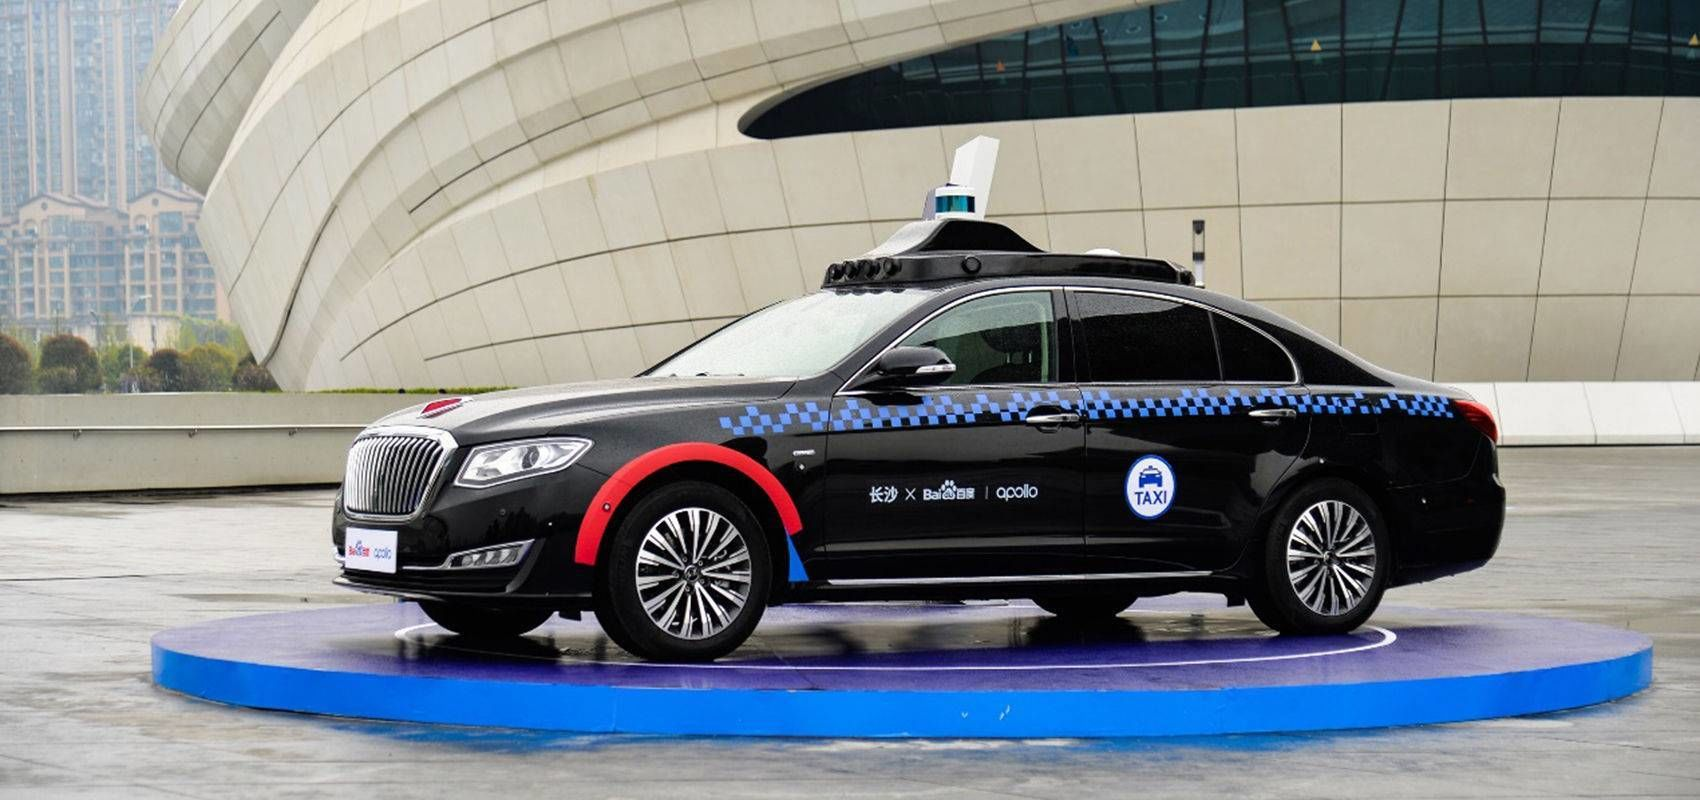
\includegraphics[width=4cm,height=3cm]{fig/apollo.jpg}
%\caption{fig1}
\end{minipage}%
}%
\subfigure[Mobileye]{
\begin{minipage}[t]{0.33\linewidth}
\centering
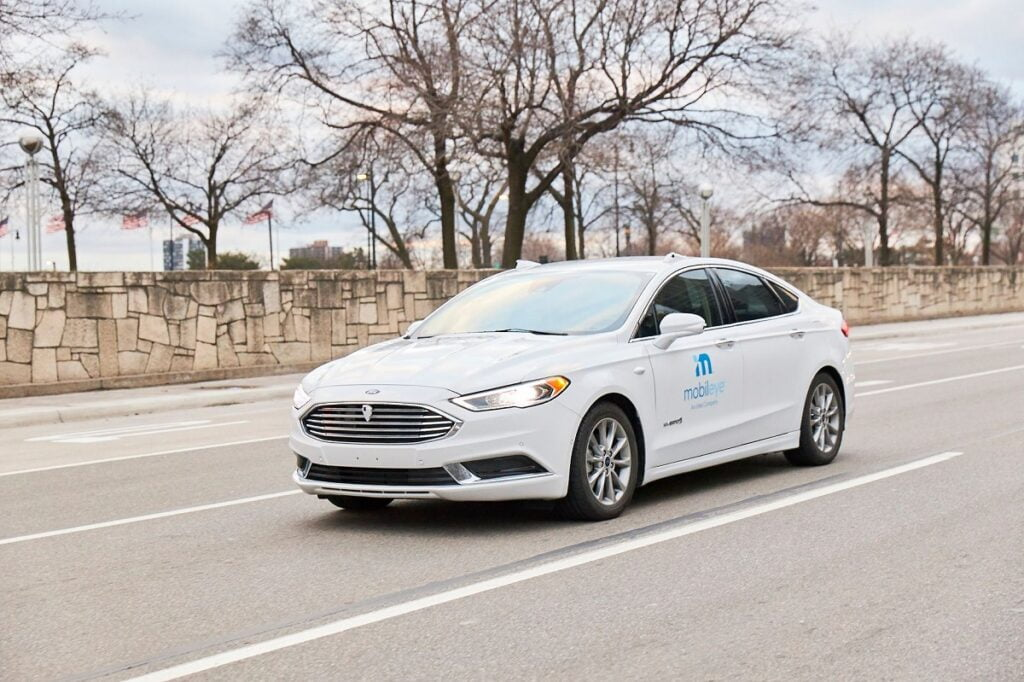
\includegraphics[width=4cm,height=3cm]{fig/mobileye.png}
%\caption{fig2}
\end{minipage}%
}%
\subfigure[Waymo]{
\begin{minipage}[t]{0.33\linewidth}
\centering
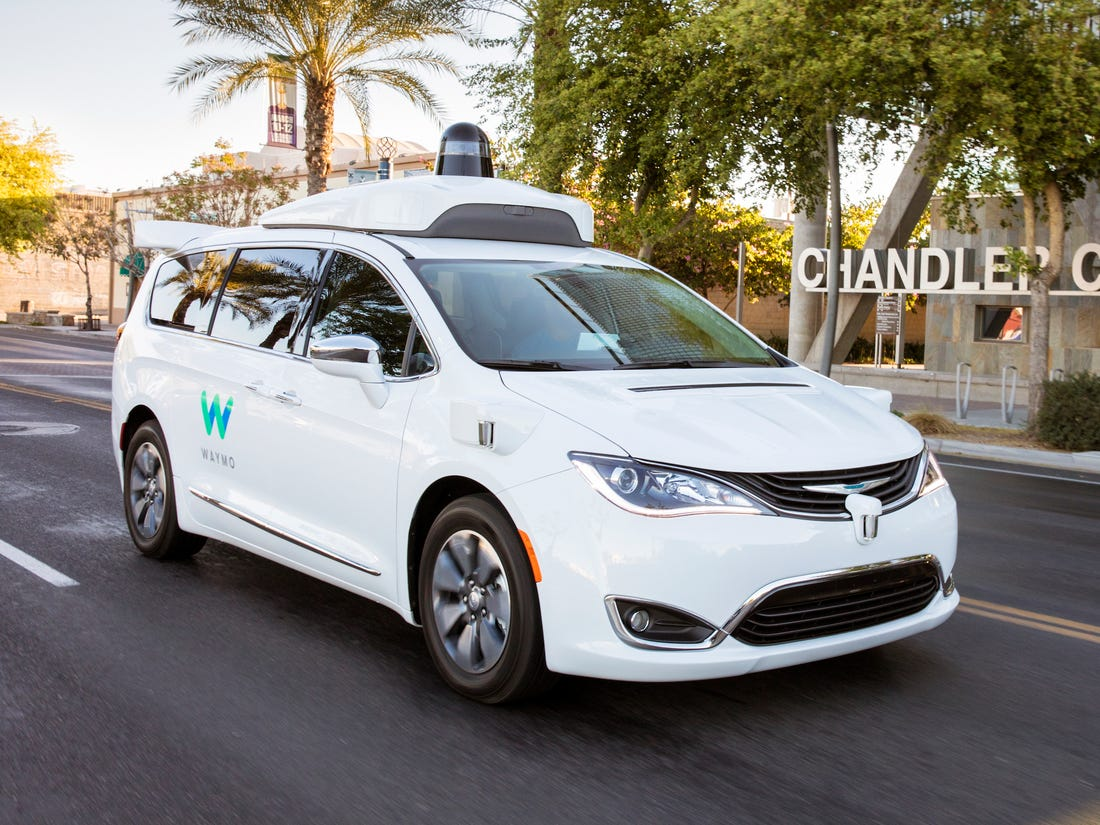
\includegraphics[width=4cm,height=3cm]{fig/waymo.jpg}
%\caption{fig2}
\end{minipage}
}%
\centering
\caption{ \textbf{无人驾驶车辆}}
\end{figure}

百度的Apollo项目特点在于其决策依赖于大量周围环境的信息,包括但不限于行人、车道线等。
在Apollo中,决策层和运动控制层有一个被称为优化层的模块,其主要作用是隔离决策层与上层模块,以减少对环境信息的依赖。虽然
Apollo已实现实用场合下的自动驾驶,例如百度在长沙进行的无人驾驶出租车测试,并已开始批量生产
无人驾驶车辆,
但是百度基于场景设计的决策模块需要与诸如智能公路这样的基础设施相结合,才能发挥出最佳效果,这点就需要与我国
优秀的基建能力相结合。

Google开发的Waymo,其特点是利用仿真器训练车辆,使其成为一个优秀的"驾驶员"。
Waymo使用自制的仿真器,其可以模拟车辆运行时的真实情况且可以创造特殊场景以供智能车训练。
。Waymo基本的技术路线是实现单车智能,即车辆的无人驾驶并不依赖于周围人造的基础设施。
Waymo遵循感知-预测-决策的系统框架。
决策组件输入感测和预测信息,并同时在设计和操作范围内
进行安全行驶。此外,Waymo的决策模块也融入了深度强化学习算法。


\subsubsection{路径规划研究现状}
路径规划广义上可划分为两种,即全局和局部。全局路径规划指在起始点和终止点之间规划出无碰轨迹。
局部路径规划,主要是指将一个个导航点输出为速度指令。下面将分别进行叙述。

(1)全局路径规划算法

全局路径规划在已知地图信息的情况下,规划出从起始点到终止点的无碰路径。按照
研究方向可以大致分为智能算法\upcite{r2,r14,r15,r22}和传统算法\upcite{r16}。

1)传统算法

 Dijkstra\upcite{r12}算法于1959 年 被提出。该算法可以找到起始点到目标点的最短路径,但缺点是运算复杂度高。
美国曼彻斯特大学的 Holland JH 教授于1967 年通过模拟生物进化和遗传理论,提
出了遗传算法\upcite{r10}并用于路径规划中。该算法的问题是可能陷入局部最优解,虽然后来有过改进,但仍不理想
。
 Hart 等人于1968 年提出启发式算法Astar \upcite{r11}算法。其作为 Dijkstra 算法的改进,可以十分高效的进行路径规划
 ,Astar 算法也一跃成为最常用的路径规划算法之一,但Astar算法在面对大尺度地图时,规划时间过长,甚至失败。
后来,人们又提出了如RA*\upcite{r8}算法以用于大尺寸地图,之后各种类似的算法如D*算法,DLite算法也都是在A*算法的基础上进行改进,
在各自擅长的方面取得了不错的效果。

2)智能算法

智能算法主要是指将机器学习的方法用于路径规划中来。如强化学习中的Qlearning算法\upcite{r13},神经网络算法等。这些算法在路径规划
中使用时,对比传统的A*\upcite{r11}等启发式算法没有明显的优势。但如Qlearning之类的智能算法,大都实现的是端到端的学习。其不需要事先知道环境地图
而是通过与外界的交互,找出路径,这点就跟人类探索环境很像。

(2)局部路径规划算法

局部路径规划将全局路径规划输出的导航点转换成速度指令,并能躲避出现在两导航点之间的动态障碍物。
这里主要介绍DWA(动态窗口法)\upcite{r21}。

DWA算法,通过在动力学允许的范围内,采样多组速度,并模拟这些速度在的相应运动轨迹
,再评价这些轨迹,选取得分最高的最优路径,并把相应的速度控制指令发送给机器人。该算法的特点在于
依据移动机器人的动力学性能限定速度采样空间在一定范围内。DWA算法之所以能成为一个广泛应用的局部路径算法,是因为
它很好的考虑到了
车辆的运动学模型,并输出了速度控制指令以到达各个导航点。

\subsubsection{深度强化学习研究现状}
强化学习\upcite{r9},简称RL,它与机器学习的其他研究领域有一定的区别,强化学习不需要专家的样本来对动作进行指导,
这是它与监督学习的区别,与非监督学习的区别在于强化学习的目的并不在于找到无任何标记的数据的背后的隐含的关系,
强化学习大都有直接的目的,如下棋游戏获得胜利等。强化学习的目的是最大化环境给予的奖励。这个过程大都满足马尔科夫性质,所以RL可以利用此性质简化计算。RL天生的决策能力再加上神经网络的抽象表达能力结合而成的深度强化学习(Deep Reforcement Learning)简称DRL
被视为是一种很有可能实现终极AI的方案。深度强化学习
按是否依赖环境模型
, 可 分 为 有 模 型RL算 法
(Model-based RL)和无模 型RL算 法(
Model-free RL )
。 深度强化学习按优化对象来 分类 , 可
分 为 基于 值 ( Value Optimization ) 和 基 于 策 略 的 优化算法
(Policy Optimization )
。 基 于 值 的  算 法 以 状 态(
state value function )或 动 作(
state-action value function )  价值 函 数  为 优化 目 标 ,通过最大化二者之一获得最优策略。 基于 策 略的算法 则直接对策 略 进行
操作,以求获得最优策略 。 这两种算法各有利弊
。基于值的算法有,Goole团队用于Atari游戏的DQN算法,其作为深度强化学习的鼻祖,为后来的研究人员指明了方向。基于策略的
算法有A3C\upcite{r5}、TRPO\upcite{r4}等。两种算法之间也可以相互结合,产生如DDPG\upcite{r6}、SAC\upcite{r3}等结合二者之长的算法\upcite{r17}。
从近年来论文发表的数量上看\upcite{r23,r24,r25,r26,r27,r28},DRL将会掀起机器学习领域新的一轮研究热潮。

\subsection{本文研究内容及篇章结构}
本文针对无人驾驶决策中存在的问题,提出使用深度强化学习中的DQN(深度Q学习)方法
来实现一个端到端的决策模块,并在Carla\upcite{r18}仿真环境中进行了车道保持任务的测试。针对传统路径规划方式无法有效的考虑人的喜好来规划路径,采用基于强化学习
的方法来进行路径规划,强化学习通过与环境的交互获得奖励,根据奖励最大化原则来规划路径,
可以通过奖励函数的个性化设计来适应每个人的需求,从而达到以人为本的路径规划。针对无人驾驶
仿真成本大的问题,本文在Carla仿真平台下进行仿真,来验证方案是否有效。
本文一共四章,每个章节的安排如下:

第一章绪论对无人驾驶领域的研究意义和基本常识做了一定介绍,通过对无人驾驶的介绍引入了无人驾驶决策部分的路径规划模块,
从而引出了利用强化学习实现“以人为本”的路径规划。通过对不同车企无人驾驶研究路线的讲述,介绍了无人驾驶目前研究现状。介绍了深度强化学习的研究现状,最后叙述了本文研究内容,并简述每章概要。

第二章对本文涉及到的决策模块进行介绍,要想设计出好的决策模块需要对无人车系统的其他部分也要有一定了解。
所以第二章介绍了无人驾驶系统的感知、决策和运动控制模块。接着介绍了本文所用无人驾驶仿真环境Carla。

第三章介绍了本文所用的强化学习路径规划算法以及深度强化学习车道保持算法。从强化学习开始讲起,详细讲述了
强化学习的相关知识,简单介绍了神经网络的知识。说明了本文所用的强化学习路径规划算法的基本原理。对本文所用
的DQN车道保持算法进行了介绍。

第四章验证了本文提出的强化学习路径规划算法和深度强化学习车道保持算法,并对实验结果进行分析与总结。包括两个部分,第一部分为使用强化学习的路径规划
采用了SARSA算法以及Q学习算法来进行路径规划,并对路径规划效果进行了分析。第二部分采用Carla仿真环境
在地图Town3中测试了基于DQN的车道保持效果,主要介绍了训练数据的预处理过程以及车道保持实验结果。

结尾部分根据本文所作工作进行总结与展望。








 \sectionend
\section{无人驾驶决策和CARLA仿真环境}

\subsection{无人驾驶技术模块概述}
无人 驾 驶经典结构由 感知 、 决 策、
控 制 三大 功能构成  。 不同的传感器和算法又组成了各种各样的子功能模块,一起构成了上述几大功能。

\subsubsection{环境感知}
环境感知作为第一环节,涵盖了定 位 、 检 测 、 目标预测。定位功 能 又可被划分为全 局定位与局部定位。全 局定 位可以凭借GPS定 位或我国的北斗导航系统来完成 , 凭此得到无人车坐标,但是一旦车辆在复 杂 的 环境条件下 
 , 上述方法定位准确性就会大幅下降 , 此时就 需要云端地 图的帮助。 智 能 车利用车 载 的 激 光 雷 达、车载 摄像机、
 各种毫米 波 雷 达来探查周边环境 , 与云端地图相匹配 , 在高清地图中确认车辆位置
 。近年来,随着深度学习算法和传统视觉处理算法的结合,仅使用视觉的环境感知模块发展迅速。
 检 测模块一般涵盖终点检测、 路人、  减速牌等环境信息的检测等。我们根据 检测物的状态是否会随时间变化,可将检测划分为静态检测和动态检测。 静态检测通常来说可
以通过自身传感器 和云端数据合作来实现 ,如识别出限速标志,障碍物等。动态检测则麻烦的多 ,因为其状态会随时间改变 , 所 以检测过程
使用了检测( Detection)-分类(Classification)-追踪(Tracking)-分割(Segmentation) 的拓扑结构 。检测 模块通常采取特定的神经网络;
 分类和追踪模块则一般采取先进的神经网络; 分割模块对输入图像进行语义分割,实现了无人车辆对所驾驶环境的感知
 ,其实现通常使用全卷积网络。
  预测功能可由两种途径完成,一种途径为使用规则,另一种途径为使用数据。使用规则 的 预测是指设计者事先对行车环境做了一定限制,即对各种现实行车环境模型
  进行建模,无人车根据这些模型输出对目标的预测
  ,由于不 可 能 枚举 所有 的行车环境,所以这种策略往往 十分脆弱 。 使用数据 的预 测一般是指
   利用前沿学科的一些方法 
  , 如使用 神经网络或其他方法得到的预 训练模 型 对周围障碍物或车道线进行预测 ,其实现目前一般采用 循环卷 积 神经 网络加上激光雷达
  分别做车道线和障碍物预测,预测结果也是两者结合的产物。
\subsubsection{行为决策}
决策 模块毫无疑问是 无 人 驾 驶车 辆的核心 , 其研究的难点在于如何在各种不确 定 的  、强耦合的 环境中 , 让 无 人
车 做 出 正 确 的 决 策  。 决策需要在不确定因素的干扰下,安全的完成任务,因此大多数决策模块采取的都是防御的策略,来确保无人车的安全。
决 策 模块大体上实现的就是路径规划的功能。

路径规划可以分为长期路径决策和局部路径决策,长期路径规划常使用迪杰斯科特或者A*算法,局部路径决策比较复杂
,需要根据感知模块的输入如交通标志的信息(比如红绿灯、车道线、限速标志等)、障碍物信息、道路结构信息等
来输出相应的动作决策和限制信息。传统的方法大都是基于规则的方法,通过对可能遇到的各种情况的枚举,输出相应
的决策,这种决策系统一旦遇到规则所没有涉及到的情况,无人车的安全性就会下降。
\subsubsection{运动控制}
运动控制模块依照决策系统的输出,再依据车辆的动力学模型 对速度指令进行滤波,将滤波后的速度指令发送到 中 心
控制 计 算机,由中心控制计算机发出具体驾驶指令, 使车辆尽 可能 的按照规定的速度与路线行驶 到目的地。

目前无人 车的运动控制有三种 方案 : 分别是PID(Proportional Integral Derivative)、 
LQR(Linear Quadratic Regulator)和
MPC(Model Predictice Control)
 。MPC控制 器突出节能特点。PID控制突出适用范围广。
LQR最优控制可以用较低的成本达到较好的控制效果。


\subsection{CARLA仿真环境}
\subsubsection{CARLA简介}
CARLA是由英特尔实验室 , 丰田研究所, UBA的计算机视觉中心研究所联合开发使用的开源免费无 人 驾 驶 仿 真平台,一经出现就因为其开源特点得到了大量支持,如今已是无人驾驶领域第一开源平台。

CARLA有很多优点,第
一个 优点是是其可以让使用者自行配置天气条件,以模拟在不同环境下的汽车的安全行驶问题,节约实际测试成本。
除此之外,开 发者也能自定义属于自己的地 图 。

CARLA第 二个优点是内置大量传感器, 例如深度、普通RGB与语义相机以及毫米波雷达等
, 并开放了PythonAPI以供使用者配置传感器属性。

CARLA第 三 个优点是其支持同步训练,即使用者可以再一个Carla环境中训练多个智能体,这个特点减少了使用者同时训练多个智能体的成本,同时也真实的模拟了实际无人驾驶情况 。 此外,CARLA
开发了ROS-bridge模块,以便于人们同时使用ROS系 统 。

CARLA也给使用者提供了无人驾驶决策的三个模板,分别是 : module-perception control pipeline(模型感知控制); end-to-end imitation learning(端到端的模仿学习), end-to-end reinforcement learning(端到端的强化学习)。 其中 ,模型感知的成 绩最好, 其 次 是 模仿学习
,强化学习排最 后 。 使用者可 以 参照这三个模板开发自己的程序。
\subsubsection{CARLA中的传感器}

在本文中主要使用了,CARLA传感器中的Semantic segmentation camera(语义分割相机),Collision detector(碰撞检测),Lane invasion detector(车道入侵检测),RGB camera(RGB相机)
故只对上述传感器进行介绍。
Semantic segmentation camera即语义相机,该摄像机通过内置的标签以不同的颜色显示物体来对可见的每个物体进行分类(例如,行人与车辆)。 
当模拟开始时,场景中的每个元素都会创建一个标签。
该相机输出的图像为R通道值为标签信息的图像:即R值为x的像素属于带有标签x的对象。具体标签信息,如表~\ref{tab:tab2}所示,在本文中为了简化训练难度,将语义相机的标签信息做了重新定义以减少训练时间。
\makeatletter% Set distance from top of page to first float
\setlength{\@fptop}{5pt}
\makeatother

\begin{table}[H]
  \centering
  \caption{\textbf{CARLA语义分割标签}}
  \begin{tabular}{lll}
    \toprule
    Value          &       Tag & 本文所用标签              \\
    \midrule
    0   & - & -\\ 
    1   & 建筑物& 行人                     \\
    2 & 栅栏& 行人    \\
    3 & 其他 & 行人 \\
    4 & 行人   & 行人     \\
    5 & 杆状物   & 其他    \\
    6 & 车道线      & 栅栏  \\
    7 & 公路    & 建筑物  \\
    8 & 人行道    & 行人    \\
    9 & 蔬菜     & 行人   \\
    10 & 车辆  & 杆状物     \\
    11& 墙    & 行人  \\
    12 & 交通标志   & 行人    \\
    \bottomrule
  \end{tabular}
  \label{tab:tab2}
\end{table}

Collision detector(碰撞检测)传感器每次在其parent actor与仿真环境中的任何事物发生碰撞时都会记录一个事件。 在单个模拟步骤中可能会检测到多个碰撞。 
为了确保检测到与任何种类的对象的冲突,服务器会为建筑物或灌木丛等元素创建"fake" actors,以便可以检索语义标签以对其进行标识。

Lane invasion detector(车道入侵检测)每次其 parent actor 超过车道标记时,都会注册一个事件。 
传感器使用地图的OPENDRIVE描述所提供的道路数据,通过考虑车轮之间的空间来确定 parent actor是否正在侵入另一个车道。

RGB camera(RGB相机)RGB摄像机充当常规摄像机,用于捕获场景中的图像。
\subsubsection{CARLA的使用}
Actors是Carla的一个核心概念,在Carla中人工创建的物体都称为Actors(演员),包括:车辆,行人,传感器等等。
而创建Actor,我们需要提供想要创建的Actor的类型,不同的类型会有不同的属性,比如一台车,它可以是不同的型号,可以是不同的颜色或外观,车辆类的actor可以通过油门和方向盘来控制,
而如果actor是一个传感器,我们需要提供传感器的类型,在车中的位置transform,也就是类似于需要使用一个模板,其在Carla中被称为蓝图,
即Blueprints,Carla中已经内置了一个蓝图库,里边包含了许多不同的Actors。

Calra的使用可以简单理解为客户端和PYTHONAPI的交互,开发者通过官方提供的PYTHONAPI样例,学习如何产生与控制actor。具体使用过程中,Carla是以python中库的
形式出现的,即只需要import carla 就可以使用python程序与Carla客户端进行交互。
Carla这种特点使得开发人员可以很方便的在Carla上验证自己的无人驾驶控制算法。

\subsection{本章小结}
本章介绍了无人驾驶系统的基本组成,通过介绍,阐述了决策模块的基本结构。
此外对本文所用的CARLA仿真环境进行了介绍,其中详细介绍了本文主要使用的传感器,并简要介绍了Calra如何使用。
 \sectionend
% \section{路径规划与车道保持算法}

\subsection{强化学习与神经网络概述}
强化学习的历史可以用两条各自独立但丰富多彩的主线来追溯。。一条主线聚焦于研究最优化控制,以及使用价
值函数动态规划等算法来寻找问题的解决方案。另一条主线源于研究动物学习心理学时产生的试错学习,对它的研究也诞生了早期 人工智能的其他领域,其一直是强化学习的主要研究内容。这两条主线在很长时间里是相对独立发展的,如今的强化学习理论主要是第二条主线的延续。如今的
强化学习主要研究这样一类问题:具有一定思考和行为能力的个体(Agent)在与其所处的环境(Environment)进行交互的过程中,
通过学习策略达到奖励最大化或实现特定的目标。其中,“个体”处在“环境”中,在某时刻可以有一个对自身的认识,这可以表示成个体自身在该时刻的状态(State)。
个体在某时刻可以向环境实施一个行为(Action),环境会因为这一行为做出相应的改变并给予个体一定形式的反馈,
个体接收到这个反馈后可以建立“自身状态”“所施行为”及“所得反馈”之间的联系,作为自身记忆的一部分给后续的决策提供参考。
个体在不同状态下向环境施加的各种不同行为则构成了个体与环境交互的“策略”(Policy)。个体策略的构建与个体的目的密切相关。
环境给予个体一个表征当前环境对个体奖惩程度的数值,我们一般称之为“奖励”(Reward)。
个体构建策略的目的就是要争取通过与环境的交互而获得尽可能多的累积奖励值。强化学习过程可用~\ref{fig:3_1}来说明。
\begin{figure}[H]
  \centering
  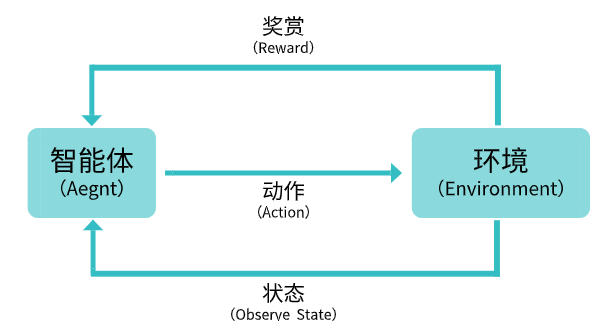
\includegraphics[width=0.5\linewidth]{fig/rl.png}
  \caption{\textbf{强化学习过程}}
  \label{fig:3_1}
\end{figure}

强化学习包括有模型强化学习和免模型强化学习,本章均会介绍。强化学习过程满足马尔科夫性。一般我们把强化学习认为是一个马尔科夫决策过程 。强化学习因为要与环境进行交互,所以会有探索与利用问题,
本章也介绍了此问题的一般解决算法即使用$\epsilon$-贪心策略来解决。
\subsubsection{$\epsilon$-贪心策略}
强化学习通过与环境的交互来累计奖励,但当agent在环境中时,就会陷入一个被称为探索利用困境的局面。
即agent如果只考虑当前奖励最大化,不去探索环境可能会错失最优解。下面通过“K-摇臂赌博机”(K-armed bandit)
问题来详细说明一下。K-摇臂赌博机(图~\ref{fig:3_2})是一种博弈类游戏工具,一台机器上有多个拉杆。赌徒拉下一个拉杆后,游戏机会随机给予一定数额的奖励。赌徒
一次只能拉下一个拉杆,每个拉杆的奖励分布是彼此独立的,即后一次拉杆奖励与前一次无关。在这个场景中,游戏机相当于环境。
个体拉下某一单臂游戏机的拉杆表示执行了一个特定的行为,游戏机会给出一个即时奖励R,随即该状态序结束。赌徒的目标是通过一定的策略
使自己获得的奖励最大化。若赌徒采取仅探索策略,即将所有机会平均分给每个摇臂,多次试验后得到每个摇臂奖励的期望,之后仅选择期望最大的摇臂。
若采用仅利用策略,即按下目前最优的(目前为止奖励最大的摇臂)摇臂。显然,“仅探索”发在估计途中,丧失了许多得到最大奖励的机会,但它较好的估算了每个摇臂的奖励
;“仅利用”发相反,它没有对摇臂奖励进行估计,选择的摇臂往往不是最优的。综上,两种方法都很难使人满意,要想达到令人满意的成果就要把二者结合起来,即在探索和利用
之间进行折中。
\begin{figure}[H]
  \centering
  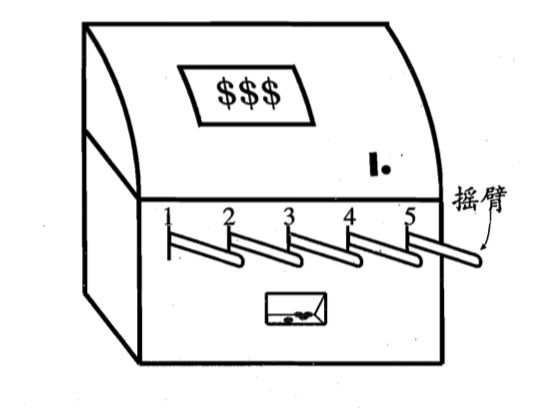
\includegraphics[width=0.6\linewidth]{fig/kab.jpg}
  \caption{\textbf{K-摇臂赌博机}}
  \label{fig:3_2}
\end{figure}

$\epsilon$-贪心策略使用一个浮动的概率来对探索和利用进行折中:每次迭代时
以$\epsilon$的概率进行探索,即以随机选择动作;以1-$\epsilon$的机率进行利用,即选择当前奖励值
最高的动作。实际程序中$\epsilon$常是一个变化的值,即在开始是$\epsilon$较大,随着与环境 交互轮数的
提升$\epsilon$越来越小。本文所用$\epsilon $贪心策略算法1所示。可以看到本文所用的$\epsilon $贪心策略是浮动变化的,开始时为一个较大的值$\epsilon_s$,最后接近于一个趋于0的值$\epsilon_e$,这样做可以很好地平衡探索与利用之间的矛盾。
\begin{algorithm}[H] 
  \caption{$\epsilon$-贪心策略}  
  \begin{algorithmic}[1] 
    \Require 起始$\epsilon$值 $\epsilon_s$ ; 终止$\epsilon$值 $\epsilon_e$ ; 
    尝试次数 T; 衰减因子 $\epsilon_d$
    \Ensure  
    \For {each $i \in T$}
      \If {$i\%Decay_{cycle}==0$}
      \State $\epsilon_d$=$\epsilon_d\times0.8$
      \EndIf
      \If {$rand()<\epsilon $}
      \State $k=from 1,2,......,K$中以均匀分布随机选取
      \Else
      \State $k=argmax_{i}Q(i)$
      \EndIf
      \State $\epsilon = \epsilon_e+(\epsilon_s- \epsilon_e)e^{\frac{-i}{\epsilon_d }}$
    \EndFor   
  \end{algorithmic}  
\end{algorithm}

\subsubsection{马尔科夫决策过程}
在一个时序过程中,如果$t+1$时的状态仅依赖于$t$时的状态$S_t$,而与$t$时之前的任何状态都无关,就定义$t$时的状态$S_t$具有马尔可夫性质(Markov Property,简称MP)。
若过程中的每一个状态均满足上述MP,则这个过程就具备MP。具备了此性质的随机过程称为马氏过程(Markov Process),简称MP
或习惯性称为马氏链(Markov Chain,简称MC)。MC可以由一个元组$<S,P>$来描述。其中$S$是有限状态集合,$P$是状态转移概率矩阵
MP的每一个状态$S_t$都仅依赖于上一个状态即状态具有完备性,而且一旦$S_t$确定了,历史状态信息$S_1,S_2,…,S_{t-1}$对于确定$S_{t+1}$就不再重要,可有可无。
用数学描述为
\begin{equation}
  P[s_{t+1}|s_t]=P[s_{t+1}|s_1,....s_t]
  \label{eq:3-1}
\end{equation}
如果一个决策过程满足MP,我们就定义这个决策过程为马尔科夫决策过程(Markov Decision Process,简称 MDP)。
至此,我们用一个$<S,A,P,R,\gamma >$来描述
一个MDP,其中$S$为有限状态集合,$A$为有限动作集合,$P$为状态转移概率矩阵,$R$为奖励函数,$\gamma $是计算累计回报时的
奖励因子。一般的MDP都对应一个策略$\pi$ ,给定策略下的累计回报如 式\eqref{eq:3-2}
\begin{equation}
  G_t=R_{t+1}+\gamma R_{t+2}+...=\sum_{k = 0}^{\infty} \gamma ^kR_{t+k+1} 
  \label{eq:3-2}
\end{equation}
我们定义在MDP中使用状态价值函数来衡量一个状态的价值,策略$\pi$下的状态
价值函数如 式\eqref{eq:3-3}
\begin{equation}
  v_\pi (s)=E_\pi [\sum_{k = 0}^{\infty}\gamma ^kR_{t+k+1}|S_t=s ]
  \label{eq:3-3}
\end{equation}
进而考虑每个动作的价值,定义动作价值函数如式 \eqref{eq:3-4}
\begin{equation}
  q_\pi (s,a)=E_\pi [\sum_{k = 0}^{\infty}\gamma ^kR_{t+k+1}|S_t=s,A_t=a ]
  \label{eq:3-4}
\end{equation}
根据MDP过程的马尔科夫性质,我们可以将式\eqref{eq:3-3}、\eqref{eq:3-4}改写为Bellman方程:
\begin{equation}
  v_\pi (s)=E_\pi [\sum_{k = 0}^{\infty}\gamma ^kR_{t+k+1}|S_t=s ]
  =E_\pi [R_{t+1}+\gamma v(S_{t+1})|S_t=s]
  \label{eq:3-5}
\end{equation}
\begin{equation}
  q_\pi (s,a)=E_\pi [\sum_{k = 0}^{\infty}\gamma ^kR_{t+k+1}|S_t=s,A_t=a ]
  =E_\pi [R_{t+1}+\gamma q(S_{t+1},A_{t+1})|S_t=s,A_t=a]
  \label{eq:3-6}
\end{equation}
给定策略$\pi $下的MDP问题可以通过其衍生的MRP(Markov Reward Process)和转移矩阵$P$来求解。由上式可知不同的策略可以得到不同的价值函数,这些价值函数之间的具有一定的不同。那么是否存在一个基于某一策略的价值函数,
在该策略下每一个状态的价值都高于其他策略?如果存在,如何找到这样的价值函数?这样的价值函数对应的策略又是什么?为了回答这些问题
,我们需要引入下述几个最优函数概念,它们之间相互对应,这也是Bellman最优递归方程的原理。

定义最优价值函数$v^*(s)$如式\eqref{eq:3-7}。最优动作值函数$q^*(s,a)$
如式\eqref{eq:3-8},即:
\begin{equation}
  v^*(s)=\max\limits_{\pi} v_\pi(s)
  \label{eq:3-7}
\end{equation}
\begin{equation}
  q^*(s,a)=\max\limits_{\pi} q_\pi(s,a)
  \label{eq:3-8}
\end{equation}
由式\eqref{eq:3-7}、\eqref{eq:3-8}可得$v^*(s)$函数和$q^*(s,a)$函数的Bellman方程
,其中$s^{'},a^{'}$分别代表下一时刻的动作和状态:
\begin{equation}
  v^*(s)=\max\limits_{a}R_s^a+\gamma \sum_{s^{'}\in{S}}P_{ss_{'}}^av^*(s^{'}) 
  \label{eq:3-9}
\end{equation}
\begin{equation}
  q^*(s,a)=R_s^a+\gamma \sum_{s^{'}\in{S}}P_{ss_{'}}^a\max\limits_{a}q^*(s^{'},a^{'}) 
  \label{eq:3-10}
\end{equation}
若已知$q^*(s,a)$,最优策略可以通过直接最大化$q^*(s,a)$来求出:
\begin{equation}
 \pi ^*(s,a)=\left\{
\begin{array}{rcl}
1       &      & {if(a=arg\max\limits_{a\in{A}} q^*(s,a))}\\
0     &      & {otherwise}\\


\end{array} \right. 
\label{eq:3-11}
\end{equation}
至此,MDP相关内容介绍完毕,其实根据Bellman最优方程可以得出最优策略,但由于Bellman最优
方程不是线性的,求解其的空间复杂度为$O(n^3)$,对于正常规模的强化学习问题无法直接求解,
且强化学习问题的环境$P$概率转移矩阵并非都是已知的,甚至大多数情况下其都是未知的。
下面就将介绍免模型学习的经典算法蒙特卡罗强化学习\upcite{r20},简称MCRL。
\subsubsection{蒙特卡罗强化学习}
在求解无模型强化学习问题 中,$P_{ss_{'}}^a$是未知的,已知的只有每一步动作的奖励以及下一个状态
。受到上文探索与利用问题的启发,可以利用一个周期内的智能体状态奖励数据,通过求取采样数据的期望来求解动作值函数,以解决环境未知带来的问题。这种方法被称为蒙特卡洛强化学习。
从下面的伪代码可以看出被评估和改进的算法都是同一个策略,因此称为同策略MC算法。
\\
\begin{algorithm}[H]  
  \caption{同策略MC法}  
  \begin{algorithmic}[1] 
    \Require 环境 E ; 动作空间 A ;
    策略执行步数 T ; 起始状态 $x_0$;
    \Ensure 
    \State $Q(s,a)=0,count(x,a)=0,\pi(x,a)=\frac{1}{|A(x)|} $ 
    \For{each $s \in T$}
    \State 在E中执行策略$\pi $产生轨迹
    \State $<x_0,a_0,r_1,a_1,r_2,.....,x_{T-1},r_T,x_T>;$
    \For{}
    \State$R=\frac{1}{T-t} \sum_{i=t+1}^{T}r_i ; $
    \State$Q(x_t,a_t)=\frac{Q(x_i,a_t)\times{count(x_t,a_t)}+R}{count(x_t,a_t)+1};$
    \State$count(x_t,a_t)=count(x_t,a_t)+1$
    \EndFor
    \State 对所有已见状态x:
    \State$$
    \pi (x)=\begin{cases}
      a=arg\max\limits_{a\in{A}} q^*(s,a)& \text{以概率1-$\epsilon$  }\\
      \text{以均匀概率从A中选取动作}& \text{以概率$\epsilon$ }
    \end{cases}
    $$
    \EndFor   
  \end{algorithmic}  
\end{algorithm}

\subsubsection{深度学习与神经网络}
深度学习(Deep Learning,简称DL)即神经网络,其通过人工神经元的相互连接让机器学会表示本身,即通过其他简单的
表示来表达复杂的表示,解决了表示学习中的核心问题。如今的人工智能浪潮,可以说就是因为深度学习的成功应用引起的。深度学习通过非线性激活函数以及隐藏层的作用,可以模拟任何函数及其导数,利用此特点,本文利用神经网络近似Q学习的值函数,下面介绍两种常见的神经网络。
\subsubsection{全连接神经网络}
全连接神经网络属于深度前馈网络的一种,下文的卷积神经网络也是深度前馈网络。全连接神经网络结构如图~\ref{fig:3-3}所示。神经网络能够拟合非线性函数的原因在于,每个神经元的非线性激活函数,常用的激活函数有sigmoid、Tanh、Relu等。本文所用激活函数
为Relu激活函数。
\begin{figure}[H]
  \centering
  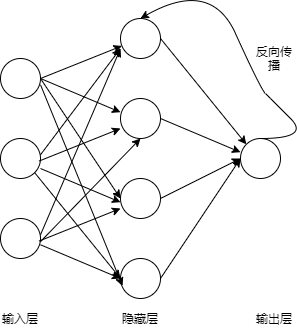
\includegraphics[width=7cm,height=7cm]{fig/mlp.png}
  \caption{\textbf{全连接神经网络}}
  \label{fig:3-3}
\end{figure}

\subsubsection{卷积神经网络}
卷积神经网络(Convolutional Neural Networks,简称 CNN),是一种使用了卷积运算的神经网络,利用卷积运算的性质,其可以很好的提取诸如图像这类矩阵类型的数据
。CNN可以说是最成功的神经网络之一,其结构如图~\ref{fig:3-4}所示。
\begin{figure}[H]
  \centering
  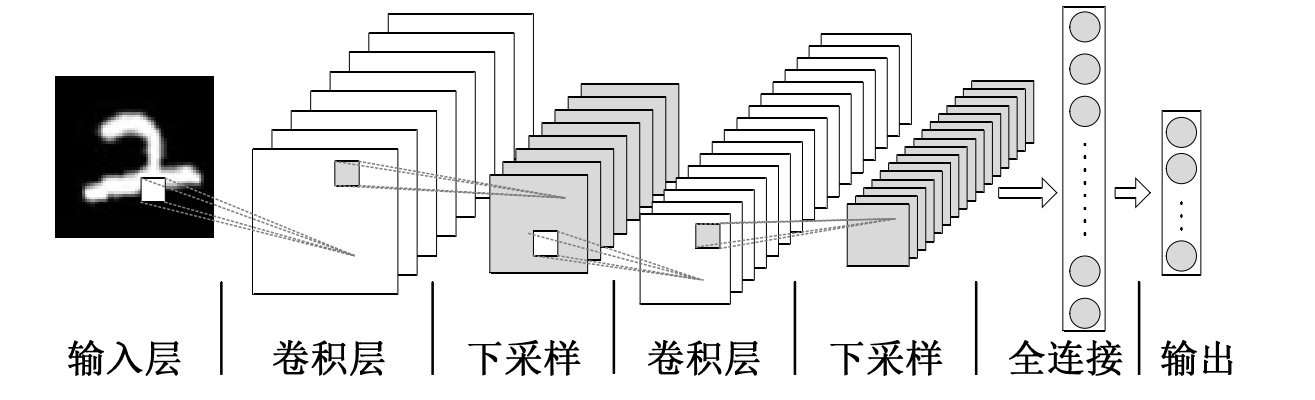
\includegraphics[width=0.9\linewidth]{fig/cnn1.png}
  \caption{\textbf{卷积神经网络}}
  \label{fig:3-4}
\end{figure}

\subsection{路径规划强化学习算法}
MC算法利用一个周期内的智能体状态奖励数据,通过求取采样数据的期望来求解动作值函数,以解决环境未知带来的问题。其缺点是运行效率较低。导致其的主要原因是MC算法没有很好地利用MDP的性质。
时序差分(Temporal-Difference Reinforcement Learning,简称TD学习)强化学习
结合了动态规划法和MC法,可以实现更高效的免模型学习,下面分别介绍同策略的TD学习(SARSA)和异策略的TD学习(Q
learning),SARSA是一个同策略算法,因为伪代码中评估(第六行),执行(第五行)的均为$\epsilon$贪心策略。
Qlearning则是异策略算法,伪代码中评估(第六行)的是原始策略,执行(第四行)的是$\epsilon$
贪心策略。本文所用的强化学习路径规划方法即这两个算法迁移到路径规划中来,并对奖励函数进行了定制处理,以满足用户需要,因为
两个算法的相似性,下面仅列出Q学习路径规划的代码。

可以看到使用Q学习进行路径规划即通过与环境交互得到当前环境下使得累计奖励最大的Q函数,通过最大化Q值函数选取路径点。Q学习的核心为其算法的更新公式即
\begin{equation}
  Q(s,a)=Q(s,a)+\alpha (r+\gamma Q(x^{'},a{'})-Q(x,a))
  \label{eq:3-12}
\end{equation}
其中$x^{'}$是前一次在状态$x$执行动作$a$转移到的状态,$a^{'}$是策略$\pi$在$x^{'}$上选择的动作;$\alpha$为学习率,其值越大
Q值收敛越快,但很可能会导致路径规划效果较差;$\gamma$为折扣因子,表示智能体的“远见程度”。$r$是指智能体执行动作$a$后所获得的奖励,
可以通过个性化设计来满足不同人的需求,可以说奖励函数的设计是强化学习任务的核心,本文的奖励函数即采用作者喜好的奖励函数,即将距离远近作为第一考虑要素。
根据Q学习更新公式,可以证明,在学习率满足0-1之间,Q学习可以
保证在无模型条件下收敛\upcite{r19}。\\
\begin{algorithm}[H]  
  \caption{SARSA}  
  \begin{algorithmic}[1] 
    \Require 环境 E ; 动作空间 A ;
     起始状态 $x_0$;折扣奖励$\gamma $;更新步长$\alpha $;
    \Ensure 
    \State $Q(s,a)=0,\pi(x,a)=\frac{1}{|A(x)|} $ ;
    \State $x=x_0,a=\pi(x);$
    \For{each $t=1,2,....do $}
    \State $r,x^{'}$=在E中执行动作a产生的奖励和转移的状态;
    \State $a^{'}=\pi^{\epsilon }(x^{'})$
    \State $Q(s,a)=Q(s,a)+\alpha (r+\gamma Q(x^{'},a{'})-Q(x,a));$
    \State $\pi(x)=arg\max_{a^{''}}Q(x,a^{''});$
    \State $x=x^{'},a=a^{'}$
    \EndFor   
  \end{algorithmic}  
\end{algorithm}

\begin{algorithm}[H]  
  \caption{Qlearning}  
  \begin{algorithmic}[1] 
    \Require 环境 E ; 动作空间 A ;
     起始状态 $x_0$;折扣奖励$\gamma $;更新步长$\alpha $;
    \Ensure 
    \State $Q(s,a)=0,\pi(x,a)=\frac{1}{|A(x)|} $ ;
    \State $x=x_0;$
    \For{each $t=1,2,....do $}
    \State $r,x^{'}$=在E中执行动作$a=\pi^{\epsilon}(x)$产生的奖励和转移的状态;
    \State $a^{'}=\pi(x^{'})$
    \State $Q(s,a)=Q(s,a)+\alpha (r+\gamma Q(x^{'},a{'})-Q(x,a));$
    \State $\pi(x)=arg\max_{a^{''}}Q(x,a^{''});$
    \State $x=x^{'}$
    \EndFor   
  \end{algorithmic}  
\end{algorithm}

\begin{algorithm}[H]  
  \caption{Qlearning路径规划}  
  \begin{algorithmic}[1] 
    \Require 环境 E ; 动作空间 A ;
     起始状态 $x_0$;折扣奖励$\gamma $;更新步长$\alpha $;迭代轮数 N;起始点和终点;
    \Ensure 
    \State $Q(s,a)=0,\pi(x,a)=\frac{1}{|A(x)|} $ ;
    \For{each $i=1,2,....Ndo $}
    \State $x=x_0;$初始化状态即回到起始点
    \For{each $t=1,2,....do $}
    \State $r,x^{'}$=在E中执行动作$a=\pi^{\epsilon}(x)$产生的奖励和转移的状态;
    \State $a^{'}=\pi(x^{'})$
    \State $Q(s,a)=Q(s,a)+\alpha (r+\gamma Q(x^{'},a{'})-Q(x,a));$
    \State $\pi(x)=arg\max_{a^{''}}Q(x,a^{''});$
    \State $x=x^{'}$
    \If{$x^{'}==end_{point}$即到达终点}
    \State $break$
    \EndIf
    \If{$x^{'}==obs$撞到障碍物}
    \State $break$
    \EndIf
    \EndFor
    \EndFor   
  \end{algorithmic}  
\end{algorithm}



\subsection{车道保持DQN算法}
DQN\upcite{r7}算法起源于2015年谷歌团队于nature上发表的Human-level control through deep reinforcement
learning。这篇论文中 提 出 的DeepQNetwork(DQN) 算法在
Atari游 戏 中 取得 了媲美人类职业玩家的成绩, DQN算法将深度神经网 络 应
用 到 强化学 习 算法 中 , 是深度强化学习的开山之作。其根据输入的 Atari 游戏屏 幕 图 片 , 选取一系列动作使得游戏得分最高。 下面将介绍DQN算法以及本文所用DQN算法框架。

\subsubsection{DQN算法原理}
DQN算法是在对传统的Q学习算法的改进上得来的,传统的Q学习算法,在面对大规模状态空间时,需要建立大规模的Q表即值函数,极其占用计算资源
研究人员称之为维度灾难。DeepMind团队DQN基本原理就是利用CNN的强大表达能力模拟Q值函数,如式\eqref{eq:3-13}
\begin{equation}
  f(s,a,w)\approx Q^*(s,a)
  \label{eq:3-13}
\end{equation}
GooleDeepMind团队DQN网络示意图如图~\ref{fig:3-5}所示,可以看到,DQN算法使用游戏屏幕图像作为输入经过
CNN的特征提取和动作输出,在Atari游戏上取得了不错的表现。
\begin{figure}[H]
  \centering
  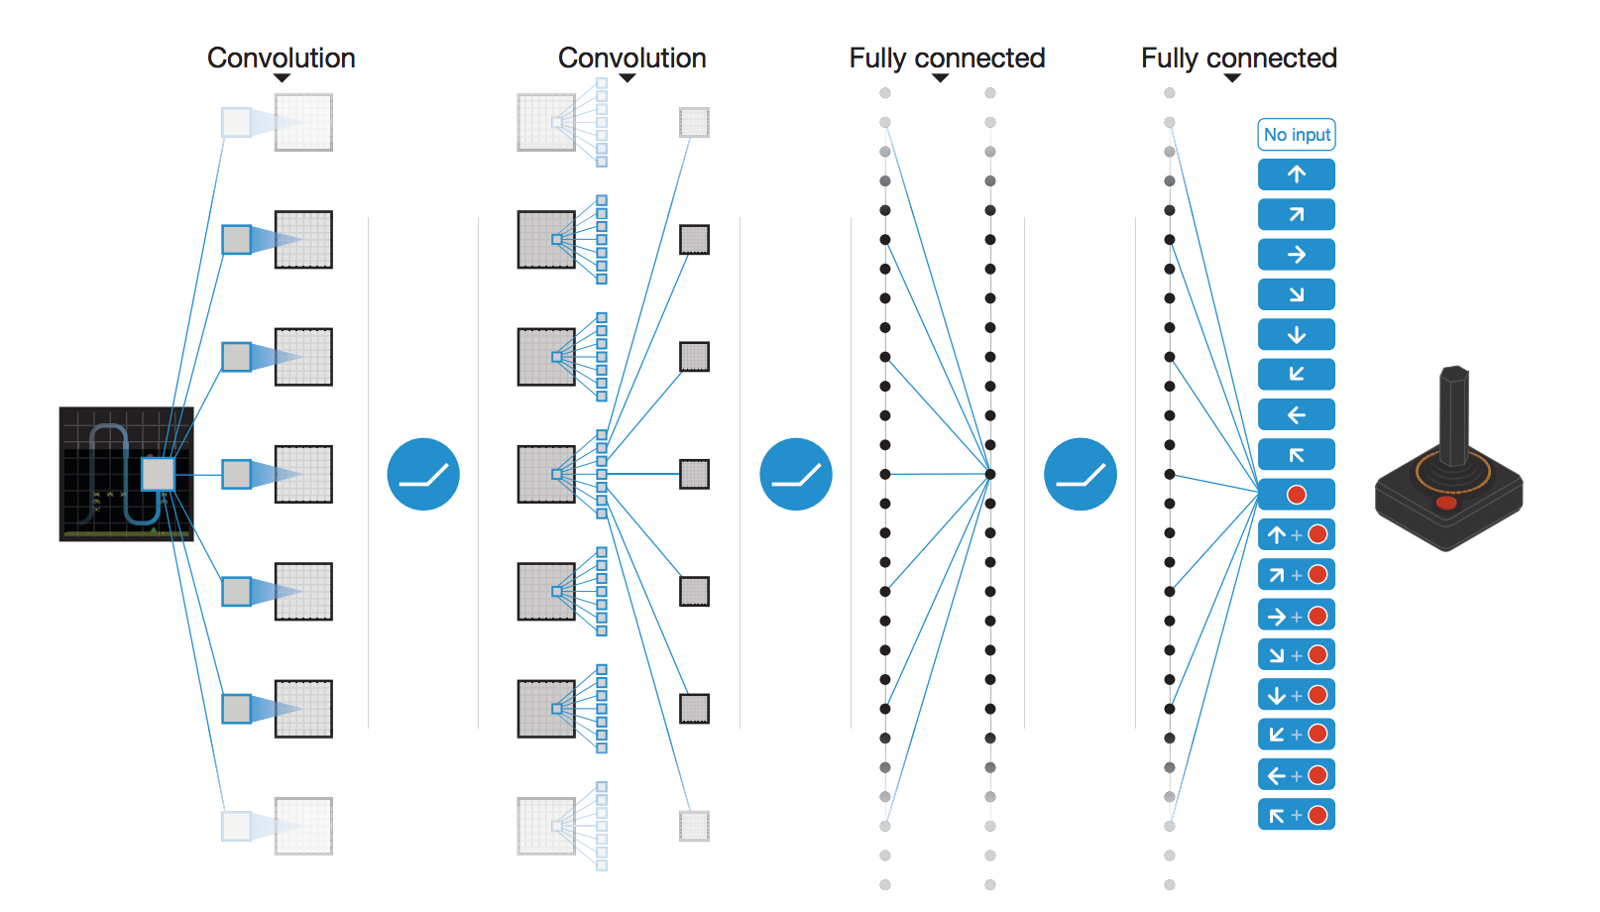
\includegraphics[width=0.9\linewidth]{fig/dqn1.png}
  \caption{\textbf{Goole团队DQN网络}}
  \label{fig:3-5}
\end{figure}

在Goole团队之前,也有研究人员使用神经网络近似Q值函数,但效果并不理想,DQN算法得以成功的具体细节如下所示:
\begin{enumerate}
  \item DQN利用CNN逼近Qlearning的$q(s,a)$即动作值函数
  \item DQN使用了经验回放机制(Experience Replay)训练智能体,经验回放机制是DQN算法获得成功的主要原因之一,DQN在于环境的迭代
   之中,前一个状态与后一个状态具有高度相关性,而神经网络要求训练数据彼此不相关,经验回放机制类似于 人类海马体的记忆原理,
   在算法中的具体体现为记录智能体与环境迭代的数据,记录数据达到一定数目后,之后就从记录的数据池中挑选数据,在喂入神经网络以打破数据之间的相关性。
  \item DQN设置双层神经网络,Qtarget和当前Q网络。两者结构相同,Qtarget网络的参数是当前Q网络参数延迟赋值得到的。在估计目标Q值时利用Qtarget网络进行估计,
  这种独特的设计减少了目标值与当前值之间的关联,是DQN获得成功的另一主要原因。
  
\end{enumerate}

DeepMind团队所用DQN算法的伪代码如下:\\
\begin{algorithm}[H]  
  \caption{使用经验回放的DQN}  
  \begin{algorithmic}
    \State 初始化 replay memory D 使用容量 N
    \State 初始化动作价值函数 $Q$ 使用随机的权重 
    \State {初始化target网络 $\hat{Q}$ 使用权重 $\theta ^{-}=\theta $ }
    \For{episode=1,M do}
    \State 初始化序列 $s_1={x_1}$ and 预处理序列 $\phi_1=\phi (s_1)$
    \For{t=1,T do}
    \State 使用可能性 $\epsilon$ 挑选随机动作 $a_t$
    \State 其他情况选择 $a_t=argmax_aQ(\phi(s_t),a;\theta)$
    \State 执行动作 $a_t$ 在仿真器并观察 $r_t$ 和图像 $x_{t+1}$
    \State 设置 $s_{t+1}=s_t,a_t,x_{t+1}$ 并且预处理$\phi_{t+1}=\phi(s_{t+1})$
    \State 存储过渡时期 $(\phi_t,a_t,r_t,\phi_{t+1})$ 在 D
    \State 在过渡时期存储库D中随机挑选样本 $(\phi_j,a_j,r_j,\phi_{j+1})$ 
    \State $$
    Set y_j=\begin{cases}
      r_j & if episode terminates at step j+1\\
      r_j+\gamma\max_{a^{'}}\hat{Q}(\phi_{j+1},a^{'};\theta^{-})&  otherwise
    \end{cases}
    $$
    \State 实施梯度下降法更新 $(y_j-Q(\phi_j,a_j;\theta))^2$其权重是网络参数 $\theta$
    \State Every C steps reset $\hat{Q}=Q$
    \EndFor 
    \EndFor
  \end{algorithmic}  
\end{algorithm}
\subsubsection{本文所用DQN算法框架}
本文所用DQN算法框架如图~\ref{fig:3-6}。
\begin{figure}[H]
  \centering
  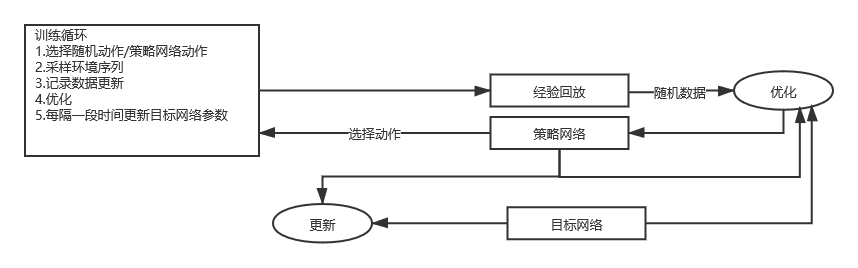
\includegraphics[width=0.7\linewidth]{fig/dqn_2.png}
  \caption{\textbf{本文所用DQN算法框架}}
  \label{fig:3-6}
\end{figure}

本文所用DQN依旧使用了CNN来 近似状态动作值函数,CNN由三个卷积层,三个BN(批处理层),一个全连接层构成。实验表明过多的神经网络层数并不能带来性能的提升,
这与强化学习探索和发现机制有关。本文的DQN网络使用Carla语义相机图片作为输入,输出为离散化的汽车控制指令,以实现一种端到端的决策模块。训练过程中也使用了Goole团队的训练技巧,包括建立双层网络,使用经验回放池,此外还对数据进行了预处理以加快训练,防止过拟合。
伪代码如下:\\
\begin{algorithm}[H]  
  \caption{DQN车道保持}  
  \begin{algorithmic}[1] 
    \Require CARLA语义相机R通道图片
    \Ensure 
    \State 初始化记忆矩阵D,初始化Q-target网络参数$w^{-}$和当前网络参数$w$
    \For{episde=1,M do}
    \State CARLA环境初始化,初始化到起点
    \For{t=1,...$T_{max}$ do}
    \State 采取上文提到的$\epsilon$贪心策略采取行动,记录$(s,a,r,s^{'})$于D
    \State 从记忆矩阵取出一批样本
    \State 用Q-target网络计算:$y=r+\gamma\max_{a^{'}}Q(s^{'},a^{'};w^{-})$
    \State 用$I=(r+\gamma\max_{a^{'}}Q(s^{'},a^{'};w^{-})-Q(s,a:w))^2$来提升参数
    \State 每隔N步将参数$w$赋值给$w^{-}$

    \EndFor
    \EndFor
     
  \end{algorithmic}  
\end{algorithm}
\subsection{本章小结}
本章介绍了强化学习和深度学习相关知识,具体介绍了本文所用的路径规划算法和车道保持算法。具体为使用Q学习和SARSA算法来进行路径规划,
并对上述方法的奖励函数进行了特别的设计,以满足用户不同的需求。除了路径规划之外,本文还将深度强化学习中的DQN算法用到车道保持任务中,仅使用Carla语义
相机输出的图片,做到车辆沿着车道行驶,避开了复杂的人工规则设计,具有一定实际价值。 \sectionend
\section{路径规划与车道保持算法}

\subsection{强化学习与神经网络概述}
强化学习的历史可以用两条各自独立但丰富多彩的主线来追溯。。一条主线聚焦于研究最优化控制,以及使用价
值函数动态规划等算法来寻找问题的解决方案。另一条主线源于研究动物学习心理学时产生的试错学习,对它的研究也诞生了早期 人工智能的其他领域,其一直是强化学习的主要研究内容。这两条主线在很长时间里是相对独立发展的,如今的强化学习理论主要是第二条主线的延续。如今的
强化学习主要研究这样一类问题:具有一定思考和行为能力的个体(Agent)在与其所处的环境(Environment)进行交互的过程中,
通过学习策略达到奖励最大化或实现特定的目标。其中,“个体”处在“环境”中,在某时刻可以有一个对自身的认识,这可以表示成个体自身在该时刻的状态(State)。
个体在某时刻可以向环境实施一个行为(Action),环境会因为这一行为做出相应的改变并给予个体一定形式的反馈,
个体接收到这个反馈后可以建立“自身状态”“所施行为”及“所得反馈”之间的联系,作为自身记忆的一部分给后续的决策提供参考。
个体在不同状态下向环境施加的各种不同行为则构成了个体与环境交互的“策略”(Policy)。个体策略的构建与个体的目的密切相关。
环境给予个体一个表征当前环境对个体奖惩程度的数值,我们一般称之为“奖励”(Reward)。
个体构建策略的目的就是要争取通过与环境的交互而获得尽可能多的累积奖励值。强化学习过程可用~\ref{fig:3_1}来说明。
\begin{figure}[H]
  \centering
  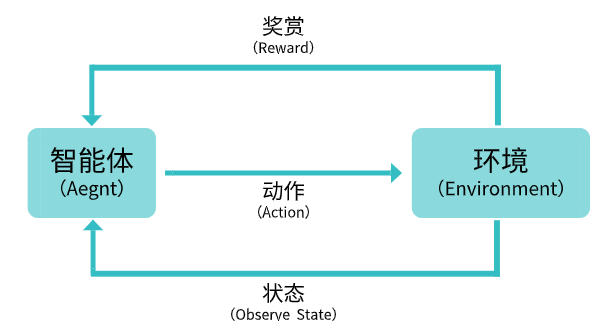
\includegraphics[width=0.5\linewidth]{fig/rl.png}
  \caption{\textbf{强化学习过程}}
  \label{fig:3_1}
\end{figure}

强化学习包括有模型强化学习和免模型强化学习,本章均会介绍。强化学习过程满足马尔科夫性。一般我们把强化学习认为是一个马尔科夫决策过程 。强化学习因为要与环境进行交互,所以会有探索与利用问题,
本章也介绍了此问题的一般解决算法即使用$\epsilon$-贪心策略来解决。
\subsubsection{$\epsilon$-贪心策略}
强化学习通过与环境的交互来累计奖励,但当agent在环境中时,就会陷入一个被称为探索利用困境的局面。
即agent如果只考虑当前奖励最大化,不去探索环境可能会错失最优解。下面通过“K-摇臂赌博机”(K-armed bandit)
问题来详细说明一下。K-摇臂赌博机(图~\ref{fig:3_2})是一种博弈类游戏工具,一台机器上有多个拉杆。赌徒拉下一个拉杆后,游戏机会随机给予一定数额的奖励。赌徒
一次只能拉下一个拉杆,每个拉杆的奖励分布是彼此独立的,即后一次拉杆奖励与前一次无关。在这个场景中,游戏机相当于环境。
个体拉下某一单臂游戏机的拉杆表示执行了一个特定的行为,游戏机会给出一个即时奖励R,随即该状态序结束。赌徒的目标是通过一定的策略
使自己获得的奖励最大化。若赌徒采取仅探索策略,即将所有机会平均分给每个摇臂,多次试验后得到每个摇臂奖励的期望,之后仅选择期望最大的摇臂。
若采用仅利用策略,即按下目前最优的(目前为止奖励最大的摇臂)摇臂。显然,“仅探索”发在估计途中,丧失了许多得到最大奖励的机会,但它较好的估算了每个摇臂的奖励
;“仅利用”发相反,它没有对摇臂奖励进行估计,选择的摇臂往往不是最优的。综上,两种方法都很难使人满意,要想达到令人满意的成果就要把二者结合起来,即在探索和利用
之间进行折中。
\begin{figure}[H]
  \centering
  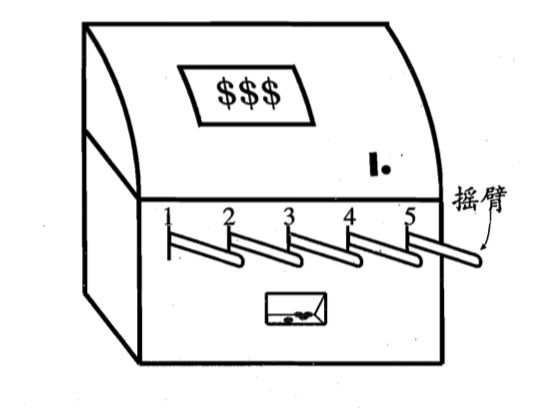
\includegraphics[width=0.6\linewidth]{fig/kab.jpg}
  \caption{\textbf{K-摇臂赌博机}}
  \label{fig:3_2}
\end{figure}

$\epsilon$-贪心策略使用一个浮动的概率来对探索和利用进行折中:每次迭代时
以$\epsilon$的概率进行探索,即以随机选择动作;以1-$\epsilon$的机率进行利用,即选择当前奖励值
最高的动作。实际程序中$\epsilon$常是一个变化的值,即在开始是$\epsilon$较大,随着与环境 交互轮数的
提升$\epsilon$越来越小。本文所用$\epsilon $贪心策略算法1所示。可以看到本文所用的$\epsilon $贪心策略是浮动变化的,开始时为一个较大的值$\epsilon_s$,最后接近于一个趋于0的值$\epsilon_e$,这样做可以很好地平衡探索与利用之间的矛盾。
\begin{algorithm}[H] 
  \caption{$\epsilon$-贪心策略}  
  \begin{algorithmic}[1] 
    \Require 起始$\epsilon$值 $\epsilon_s$ ; 终止$\epsilon$值 $\epsilon_e$ ; 
    尝试次数 T; 衰减因子 $\epsilon_d$
    \Ensure  
    \For {each $i \in T$}
      \If {$i\%Decay_{cycle}==0$}
      \State $\epsilon_d$=$\epsilon_d\times0.8$
      \EndIf
      \If {$rand()<\epsilon $}
      \State $k=from 1,2,......,K$中以均匀分布随机选取
      \Else
      \State $k=argmax_{i}Q(i)$
      \EndIf
      \State $\epsilon = \epsilon_e+(\epsilon_s- \epsilon_e)e^{\frac{-i}{\epsilon_d }}$
    \EndFor   
  \end{algorithmic}  
\end{algorithm}

\subsubsection{马尔科夫决策过程}
在一个时序过程中,如果$t+1$时的状态仅依赖于$t$时的状态$S_t$,而与$t$时之前的任何状态都无关,就定义$t$时的状态$S_t$具有马尔可夫性质(Markov Property,简称MP)。
若过程中的每一个状态均满足上述MP,则这个过程就具备MP。具备了此性质的随机过程称为马氏过程(Markov Process),简称MP
或习惯性称为马氏链(Markov Chain,简称MC)。MC可以由一个元组$<S,P>$来描述。其中$S$是有限状态集合,$P$是状态转移概率矩阵
MP的每一个状态$S_t$都仅依赖于上一个状态即状态具有完备性,而且一旦$S_t$确定了,历史状态信息$S_1,S_2,…,S_{t-1}$对于确定$S_{t+1}$就不再重要,可有可无。
用数学描述为
\begin{equation}
  P[s_{t+1}|s_t]=P[s_{t+1}|s_1,....s_t]
  \label{eq:3-1}
\end{equation}
如果一个决策过程满足MP,我们就定义这个决策过程为马尔科夫决策过程(Markov Decision Process,简称 MDP)。
至此,我们用一个$<S,A,P,R,\gamma >$来描述
一个MDP,其中$S$为有限状态集合,$A$为有限动作集合,$P$为状态转移概率矩阵,$R$为奖励函数,$\gamma $是计算累计回报时的
奖励因子。一般的MDP都对应一个策略$\pi$ ,给定策略下的累计回报如 式\eqref{eq:3-2}
\begin{equation}
  G_t=R_{t+1}+\gamma R_{t+2}+...=\sum_{k = 0}^{\infty} \gamma ^kR_{t+k+1} 
  \label{eq:3-2}
\end{equation}
我们定义在MDP中使用状态价值函数来衡量一个状态的价值,策略$\pi$下的状态
价值函数如 式\eqref{eq:3-3}
\begin{equation}
  v_\pi (s)=E_\pi [\sum_{k = 0}^{\infty}\gamma ^kR_{t+k+1}|S_t=s ]
  \label{eq:3-3}
\end{equation}
进而考虑每个动作的价值,定义动作价值函数如式 \eqref{eq:3-4}
\begin{equation}
  q_\pi (s,a)=E_\pi [\sum_{k = 0}^{\infty}\gamma ^kR_{t+k+1}|S_t=s,A_t=a ]
  \label{eq:3-4}
\end{equation}
根据MDP过程的马尔科夫性质,我们可以将式\eqref{eq:3-3}、\eqref{eq:3-4}改写为Bellman方程:
\begin{equation}
  v_\pi (s)=E_\pi [\sum_{k = 0}^{\infty}\gamma ^kR_{t+k+1}|S_t=s ]
  =E_\pi [R_{t+1}+\gamma v(S_{t+1})|S_t=s]
  \label{eq:3-5}
\end{equation}
\begin{equation}
  q_\pi (s,a)=E_\pi [\sum_{k = 0}^{\infty}\gamma ^kR_{t+k+1}|S_t=s,A_t=a ]
  =E_\pi [R_{t+1}+\gamma q(S_{t+1},A_{t+1})|S_t=s,A_t=a]
  \label{eq:3-6}
\end{equation}
给定策略$\pi $下的MDP问题可以通过其衍生的MRP(Markov Reward Process)和转移矩阵$P$来求解。由上式可知不同的策略可以得到不同的价值函数,这些价值函数之间的具有一定的不同。那么是否存在一个基于某一策略的价值函数,
在该策略下每一个状态的价值都高于其他策略?如果存在,如何找到这样的价值函数?这样的价值函数对应的策略又是什么?为了回答这些问题
,我们需要引入下述几个最优函数概念,它们之间相互对应,这也是Bellman最优递归方程的原理。

定义最优价值函数$v^*(s)$如式\eqref{eq:3-7}。最优动作值函数$q^*(s,a)$
如式\eqref{eq:3-8},即:
\begin{equation}
  v^*(s)=\max\limits_{\pi} v_\pi(s)
  \label{eq:3-7}
\end{equation}
\begin{equation}
  q^*(s,a)=\max\limits_{\pi} q_\pi(s,a)
  \label{eq:3-8}
\end{equation}
由式\eqref{eq:3-7}、\eqref{eq:3-8}可得$v^*(s)$函数和$q^*(s,a)$函数的Bellman方程
,其中$s^{'},a^{'}$分别代表下一时刻的动作和状态:
\begin{equation}
  v^*(s)=\max\limits_{a}R_s^a+\gamma \sum_{s^{'}\in{S}}P_{ss_{'}}^av^*(s^{'}) 
  \label{eq:3-9}
\end{equation}
\begin{equation}
  q^*(s,a)=R_s^a+\gamma \sum_{s^{'}\in{S}}P_{ss_{'}}^a\max\limits_{a}q^*(s^{'},a^{'}) 
  \label{eq:3-10}
\end{equation}
若已知$q^*(s,a)$,最优策略可以通过直接最大化$q^*(s,a)$来求出:
\begin{equation}
 \pi ^*(s,a)=\left\{
\begin{array}{rcl}
1       &      & {if(a=arg\max\limits_{a\in{A}} q^*(s,a))}\\
0     &      & {otherwise}\\


\end{array} \right. 
\label{eq:3-11}
\end{equation}
至此,MDP相关内容介绍完毕,其实根据Bellman最优方程可以得出最优策略,但由于Bellman最优
方程不是线性的,求解其的空间复杂度为$O(n^3)$,对于正常规模的强化学习问题无法直接求解,
且强化学习问题的环境$P$概率转移矩阵并非都是已知的,甚至大多数情况下其都是未知的。
下面就将介绍免模型学习的经典算法蒙特卡罗强化学习\upcite{r20},简称MCRL。
\subsubsection{蒙特卡罗强化学习}
在求解无模型强化学习问题 中,$P_{ss_{'}}^a$是未知的,已知的只有每一步动作的奖励以及下一个状态
。受到上文探索与利用问题的启发,可以利用一个周期内的智能体状态奖励数据,通过求取采样数据的期望来求解动作值函数,以解决环境未知带来的问题。这种方法被称为蒙特卡洛强化学习。
从下面的伪代码可以看出被评估和改进的算法都是同一个策略,因此称为同策略MC算法。
\\
\begin{algorithm}[H]  
  \caption{同策略MC法}  
  \begin{algorithmic}[1] 
    \Require 环境 E ; 动作空间 A ;
    策略执行步数 T ; 起始状态 $x_0$;
    \Ensure 
    \State $Q(s,a)=0,count(x,a)=0,\pi(x,a)=\frac{1}{|A(x)|} $ 
    \For{each $s \in T$}
    \State 在E中执行策略$\pi $产生轨迹
    \State $<x_0,a_0,r_1,a_1,r_2,.....,x_{T-1},r_T,x_T>;$
    \For{}
    \State$R=\frac{1}{T-t} \sum_{i=t+1}^{T}r_i ; $
    \State$Q(x_t,a_t)=\frac{Q(x_i,a_t)\times{count(x_t,a_t)}+R}{count(x_t,a_t)+1};$
    \State$count(x_t,a_t)=count(x_t,a_t)+1$
    \EndFor
    \State 对所有已见状态x:
    \State$$
    \pi (x)=\begin{cases}
      a=arg\max\limits_{a\in{A}} q^*(s,a)& \text{以概率1-$\epsilon$  }\\
      \text{以均匀概率从A中选取动作}& \text{以概率$\epsilon$ }
    \end{cases}
    $$
    \EndFor   
  \end{algorithmic}  
\end{algorithm}

\subsubsection{深度学习与神经网络}
深度学习(Deep Learning,简称DL)即神经网络,其通过人工神经元的相互连接让机器学会表示本身,即通过其他简单的
表示来表达复杂的表示,解决了表示学习中的核心问题。如今的人工智能浪潮,可以说就是因为深度学习的成功应用引起的。深度学习通过非线性激活函数以及隐藏层的作用,可以模拟任何函数及其导数,利用此特点,本文利用神经网络近似Q学习的值函数,下面介绍两种常见的神经网络。
\subsubsection{全连接神经网络}
全连接神经网络属于深度前馈网络的一种,下文的卷积神经网络也是深度前馈网络。全连接神经网络结构如图~\ref{fig:3-3}所示。神经网络能够拟合非线性函数的原因在于,每个神经元的非线性激活函数,常用的激活函数有sigmoid、Tanh、Relu等。本文所用激活函数
为Relu激活函数。
\begin{figure}[H]
  \centering
  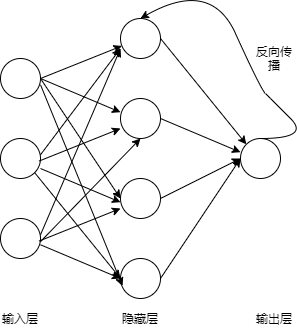
\includegraphics[width=7cm,height=7cm]{fig/mlp.png}
  \caption{\textbf{全连接神经网络}}
  \label{fig:3-3}
\end{figure}

\subsubsection{卷积神经网络}
卷积神经网络(Convolutional Neural Networks,简称 CNN),是一种使用了卷积运算的神经网络,利用卷积运算的性质,其可以很好的提取诸如图像这类矩阵类型的数据
。CNN可以说是最成功的神经网络之一,其结构如图~\ref{fig:3-4}所示。
\begin{figure}[H]
  \centering
  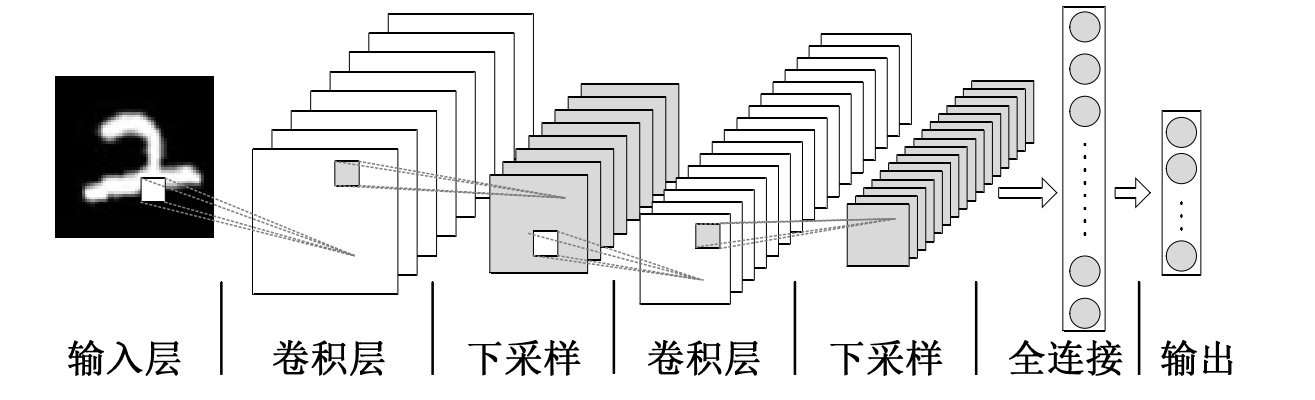
\includegraphics[width=0.9\linewidth]{fig/cnn1.png}
  \caption{\textbf{卷积神经网络}}
  \label{fig:3-4}
\end{figure}

\subsection{路径规划强化学习算法}
MC算法利用一个周期内的智能体状态奖励数据,通过求取采样数据的期望来求解动作值函数,以解决环境未知带来的问题。其缺点是运行效率较低。导致其的主要原因是MC算法没有很好地利用MDP的性质。
时序差分(Temporal-Difference Reinforcement Learning,简称TD学习)强化学习
结合了动态规划法和MC法,可以实现更高效的免模型学习,下面分别介绍同策略的TD学习(SARSA)和异策略的TD学习(Q
learning),SARSA是一个同策略算法,因为伪代码中评估(第六行),执行(第五行)的均为$\epsilon$贪心策略。
Qlearning则是异策略算法,伪代码中评估(第六行)的是原始策略,执行(第四行)的是$\epsilon$
贪心策略。本文所用的强化学习路径规划方法即这两个算法迁移到路径规划中来,并对奖励函数进行了定制处理,以满足用户需要,因为
两个算法的相似性,下面仅列出Q学习路径规划的代码。

可以看到使用Q学习进行路径规划即通过与环境交互得到当前环境下使得累计奖励最大的Q函数,通过最大化Q值函数选取路径点。Q学习的核心为其算法的更新公式即
\begin{equation}
  Q(s,a)=Q(s,a)+\alpha (r+\gamma Q(x^{'},a{'})-Q(x,a))
  \label{eq:3-12}
\end{equation}
其中$x^{'}$是前一次在状态$x$执行动作$a$转移到的状态,$a^{'}$是策略$\pi$在$x^{'}$上选择的动作;$\alpha$为学习率,其值越大
Q值收敛越快,但很可能会导致路径规划效果较差;$\gamma$为折扣因子,表示智能体的“远见程度”。$r$是指智能体执行动作$a$后所获得的奖励,
可以通过个性化设计来满足不同人的需求,可以说奖励函数的设计是强化学习任务的核心,本文的奖励函数即采用作者喜好的奖励函数,即将距离远近作为第一考虑要素。
根据Q学习更新公式,可以证明,在学习率满足0-1之间,Q学习可以
保证在无模型条件下收敛\upcite{r19}。\\
\begin{algorithm}[H]  
  \caption{SARSA}  
  \begin{algorithmic}[1] 
    \Require 环境 E ; 动作空间 A ;
     起始状态 $x_0$;折扣奖励$\gamma $;更新步长$\alpha $;
    \Ensure 
    \State $Q(s,a)=0,\pi(x,a)=\frac{1}{|A(x)|} $ ;
    \State $x=x_0,a=\pi(x);$
    \For{each $t=1,2,....do $}
    \State $r,x^{'}$=在E中执行动作a产生的奖励和转移的状态;
    \State $a^{'}=\pi^{\epsilon }(x^{'})$
    \State $Q(s,a)=Q(s,a)+\alpha (r+\gamma Q(x^{'},a{'})-Q(x,a));$
    \State $\pi(x)=arg\max_{a^{''}}Q(x,a^{''});$
    \State $x=x^{'},a=a^{'}$
    \EndFor   
  \end{algorithmic}  
\end{algorithm}

\begin{algorithm}[H]  
  \caption{Qlearning}  
  \begin{algorithmic}[1] 
    \Require 环境 E ; 动作空间 A ;
     起始状态 $x_0$;折扣奖励$\gamma $;更新步长$\alpha $;
    \Ensure 
    \State $Q(s,a)=0,\pi(x,a)=\frac{1}{|A(x)|} $ ;
    \State $x=x_0;$
    \For{each $t=1,2,....do $}
    \State $r,x^{'}$=在E中执行动作$a=\pi^{\epsilon}(x)$产生的奖励和转移的状态;
    \State $a^{'}=\pi(x^{'})$
    \State $Q(s,a)=Q(s,a)+\alpha (r+\gamma Q(x^{'},a{'})-Q(x,a));$
    \State $\pi(x)=arg\max_{a^{''}}Q(x,a^{''});$
    \State $x=x^{'}$
    \EndFor   
  \end{algorithmic}  
\end{algorithm}

\begin{algorithm}[H]  
  \caption{Qlearning路径规划}  
  \begin{algorithmic}[1] 
    \Require 环境 E ; 动作空间 A ;
     起始状态 $x_0$;折扣奖励$\gamma $;更新步长$\alpha $;迭代轮数 N;起始点和终点;
    \Ensure 
    \State $Q(s,a)=0,\pi(x,a)=\frac{1}{|A(x)|} $ ;
    \For{each $i=1,2,....Ndo $}
    \State $x=x_0;$初始化状态即回到起始点
    \For{each $t=1,2,....do $}
    \State $r,x^{'}$=在E中执行动作$a=\pi^{\epsilon}(x)$产生的奖励和转移的状态;
    \State $a^{'}=\pi(x^{'})$
    \State $Q(s,a)=Q(s,a)+\alpha (r+\gamma Q(x^{'},a{'})-Q(x,a));$
    \State $\pi(x)=arg\max_{a^{''}}Q(x,a^{''});$
    \State $x=x^{'}$
    \If{$x^{'}==end_{point}$即到达终点}
    \State $break$
    \EndIf
    \If{$x^{'}==obs$撞到障碍物}
    \State $break$
    \EndIf
    \EndFor
    \EndFor   
  \end{algorithmic}  
\end{algorithm}



\subsection{车道保持DQN算法}
DQN\upcite{r7}算法起源于2015年谷歌团队于nature上发表的Human-level control through deep reinforcement
learning。这篇论文中 提 出 的DeepQNetwork(DQN) 算法在
Atari游 戏 中 取得 了媲美人类职业玩家的成绩, DQN算法将深度神经网 络 应
用 到 强化学 习 算法 中 , 是深度强化学习的开山之作。其根据输入的 Atari 游戏屏 幕 图 片 , 选取一系列动作使得游戏得分最高。 下面将介绍DQN算法以及本文所用DQN算法框架。

\subsubsection{DQN算法原理}
DQN算法是在对传统的Q学习算法的改进上得来的,传统的Q学习算法,在面对大规模状态空间时,需要建立大规模的Q表即值函数,极其占用计算资源
研究人员称之为维度灾难。DeepMind团队DQN基本原理就是利用CNN的强大表达能力模拟Q值函数,如式\eqref{eq:3-13}
\begin{equation}
  f(s,a,w)\approx Q^*(s,a)
  \label{eq:3-13}
\end{equation}
GooleDeepMind团队DQN网络示意图如图~\ref{fig:3-5}所示,可以看到,DQN算法使用游戏屏幕图像作为输入经过
CNN的特征提取和动作输出,在Atari游戏上取得了不错的表现。
\begin{figure}[H]
  \centering
  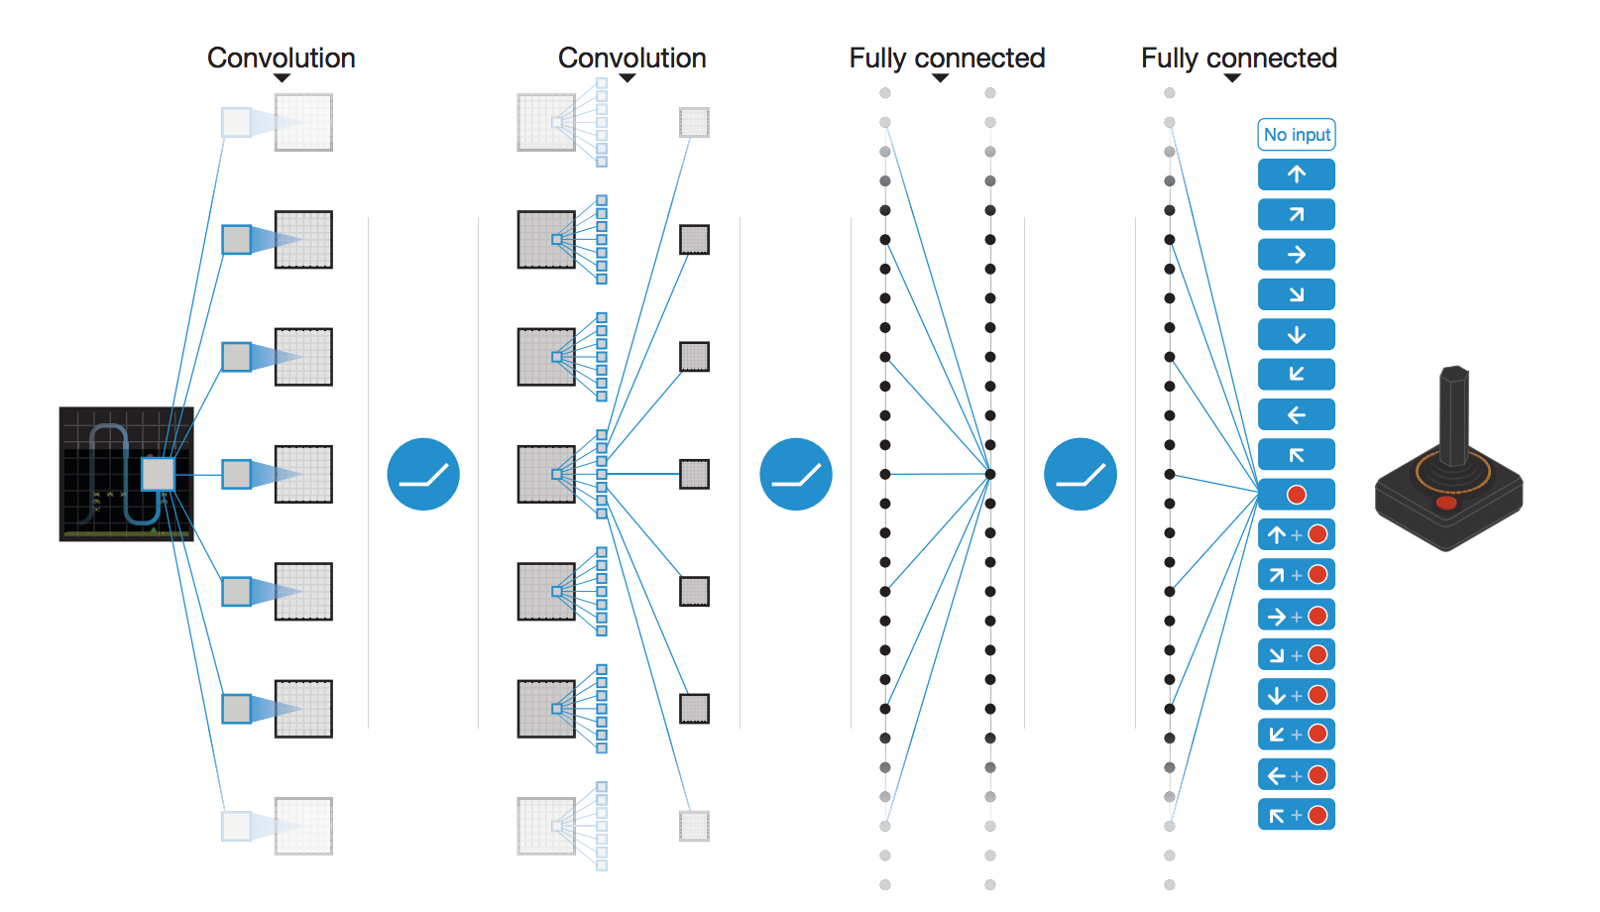
\includegraphics[width=0.9\linewidth]{fig/dqn1.png}
  \caption{\textbf{Goole团队DQN网络}}
  \label{fig:3-5}
\end{figure}

在Goole团队之前,也有研究人员使用神经网络近似Q值函数,但效果并不理想,DQN算法得以成功的具体细节如下所示:
\begin{enumerate}
  \item DQN利用CNN逼近Qlearning的$q(s,a)$即动作值函数
  \item DQN使用了经验回放机制(Experience Replay)训练智能体,经验回放机制是DQN算法获得成功的主要原因之一,DQN在于环境的迭代
   之中,前一个状态与后一个状态具有高度相关性,而神经网络要求训练数据彼此不相关,经验回放机制类似于 人类海马体的记忆原理,
   在算法中的具体体现为记录智能体与环境迭代的数据,记录数据达到一定数目后,之后就从记录的数据池中挑选数据,在喂入神经网络以打破数据之间的相关性。
  \item DQN设置双层神经网络,Qtarget和当前Q网络。两者结构相同,Qtarget网络的参数是当前Q网络参数延迟赋值得到的。在估计目标Q值时利用Qtarget网络进行估计,
  这种独特的设计减少了目标值与当前值之间的关联,是DQN获得成功的另一主要原因。
  
\end{enumerate}

DeepMind团队所用DQN算法的伪代码如下:\\
\begin{algorithm}[H]  
  \caption{使用经验回放的DQN}  
  \begin{algorithmic}
    \State 初始化 replay memory D 使用容量 N
    \State 初始化动作价值函数 $Q$ 使用随机的权重 
    \State {初始化target网络 $\hat{Q}$ 使用权重 $\theta ^{-}=\theta $ }
    \For{episode=1,M do}
    \State 初始化序列 $s_1={x_1}$ and 预处理序列 $\phi_1=\phi (s_1)$
    \For{t=1,T do}
    \State 使用可能性 $\epsilon$ 挑选随机动作 $a_t$
    \State 其他情况选择 $a_t=argmax_aQ(\phi(s_t),a;\theta)$
    \State 执行动作 $a_t$ 在仿真器并观察 $r_t$ 和图像 $x_{t+1}$
    \State 设置 $s_{t+1}=s_t,a_t,x_{t+1}$ 并且预处理$\phi_{t+1}=\phi(s_{t+1})$
    \State 存储过渡时期 $(\phi_t,a_t,r_t,\phi_{t+1})$ 在 D
    \State 在过渡时期存储库D中随机挑选样本 $(\phi_j,a_j,r_j,\phi_{j+1})$ 
    \State $$
    Set y_j=\begin{cases}
      r_j & if episode terminates at step j+1\\
      r_j+\gamma\max_{a^{'}}\hat{Q}(\phi_{j+1},a^{'};\theta^{-})&  otherwise
    \end{cases}
    $$
    \State 实施梯度下降法更新 $(y_j-Q(\phi_j,a_j;\theta))^2$其权重是网络参数 $\theta$
    \State Every C steps reset $\hat{Q}=Q$
    \EndFor 
    \EndFor
  \end{algorithmic}  
\end{algorithm}
\subsubsection{本文所用DQN算法框架}
本文所用DQN算法框架如图~\ref{fig:3-6}。
\begin{figure}[H]
  \centering
  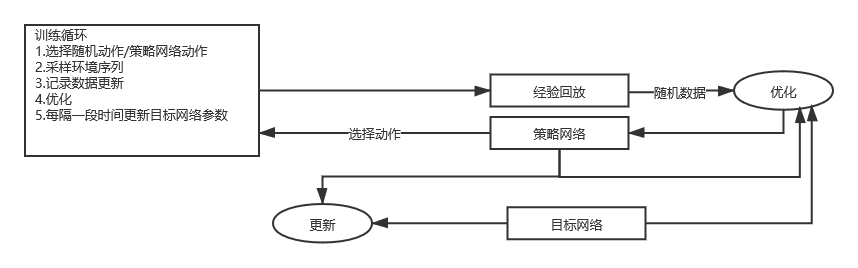
\includegraphics[width=0.7\linewidth]{fig/dqn_2.png}
  \caption{\textbf{本文所用DQN算法框架}}
  \label{fig:3-6}
\end{figure}

本文所用DQN依旧使用了CNN来 近似状态动作值函数,CNN由三个卷积层,三个BN(批处理层),一个全连接层构成。实验表明过多的神经网络层数并不能带来性能的提升,
这与强化学习探索和发现机制有关。本文的DQN网络使用Carla语义相机图片作为输入,输出为离散化的汽车控制指令,以实现一种端到端的决策模块。训练过程中也使用了Goole团队的训练技巧,包括建立双层网络,使用经验回放池,此外还对数据进行了预处理以加快训练,防止过拟合。
伪代码如下:\\
\begin{algorithm}[H]  
  \caption{DQN车道保持}  
  \begin{algorithmic}[1] 
    \Require CARLA语义相机R通道图片
    \Ensure 
    \State 初始化记忆矩阵D,初始化Q-target网络参数$w^{-}$和当前网络参数$w$
    \For{episde=1,M do}
    \State CARLA环境初始化,初始化到起点
    \For{t=1,...$T_{max}$ do}
    \State 采取上文提到的$\epsilon$贪心策略采取行动,记录$(s,a,r,s^{'})$于D
    \State 从记忆矩阵取出一批样本
    \State 用Q-target网络计算:$y=r+\gamma\max_{a^{'}}Q(s^{'},a^{'};w^{-})$
    \State 用$I=(r+\gamma\max_{a^{'}}Q(s^{'},a^{'};w^{-})-Q(s,a:w))^2$来提升参数
    \State 每隔N步将参数$w$赋值给$w^{-}$

    \EndFor
    \EndFor
     
  \end{algorithmic}  
\end{algorithm}
\subsection{本章小结}
本章介绍了强化学习和深度学习相关知识,具体介绍了本文所用的路径规划算法和车道保持算法。具体为使用Q学习和SARSA算法来进行路径规划,
并对上述方法的奖励函数进行了特别的设计,以满足用户不同的需求。除了路径规划之外,本文还将深度强化学习中的DQN算法用到车道保持任务中,仅使用Carla语义
相机输出的图片,做到车辆沿着车道行驶,避开了复杂的人工规则设计,具有一定实际价值。 \sectionend
\section{仿真实验与分析}
本章介绍了在Ubuntu系统下本文使用的强化学习路径规划和深度强化学习车道保持算法实验结果,具体内容如下所示。
\subsection{路径规划仿真}
\subsubsection{仿真环境}
路径规划仿真所用环境为Python+gym,gym为Python强化学习库。具体为使用Ubuntu20.04系统,在Pycharm中利用Python建立了一个gym风格的环境来进行强化学习
路径规划。此环境可以理解为供强化学习进行迭代训练的“地图”,在这个环境中智能体每做出一个动作,环境都会给出在当前状态下的奖励。
对于强化学习而言此环境是必须的,在本文的程序中,奖励函数在环境中给出。
\subsubsection{Qlearning路径规划}
Qlearning路径规划效果图
如图~\ref{fig:4-1}。
\begin{figure}[H]
  \centering
  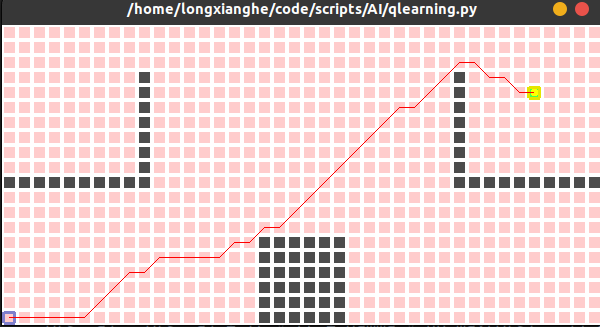
\includegraphics[width=0.8\linewidth]{fig/qlearning.png}
  \caption{\textbf{Q-leaning路径规划}}
  \label{fig:4-1}
\end{figure}
可以看到基于Qlearning算法可以成功规划出路径,此路径对比最短路径差距不大,且可以通过定制
奖励函数的方式,实现基于 用户的个性化路径规划。因为本文所用的奖励函数的原则为距离的远近,
所以可以看出路线中较多的使用了直线,拐弯集中发生于障碍物附近。由此可以看出采用Q学习的算法
,路径规划的结果可以达到设计之初的要求,这与强化学习的机制有关。
\begin{figure}[H]
  \centering
  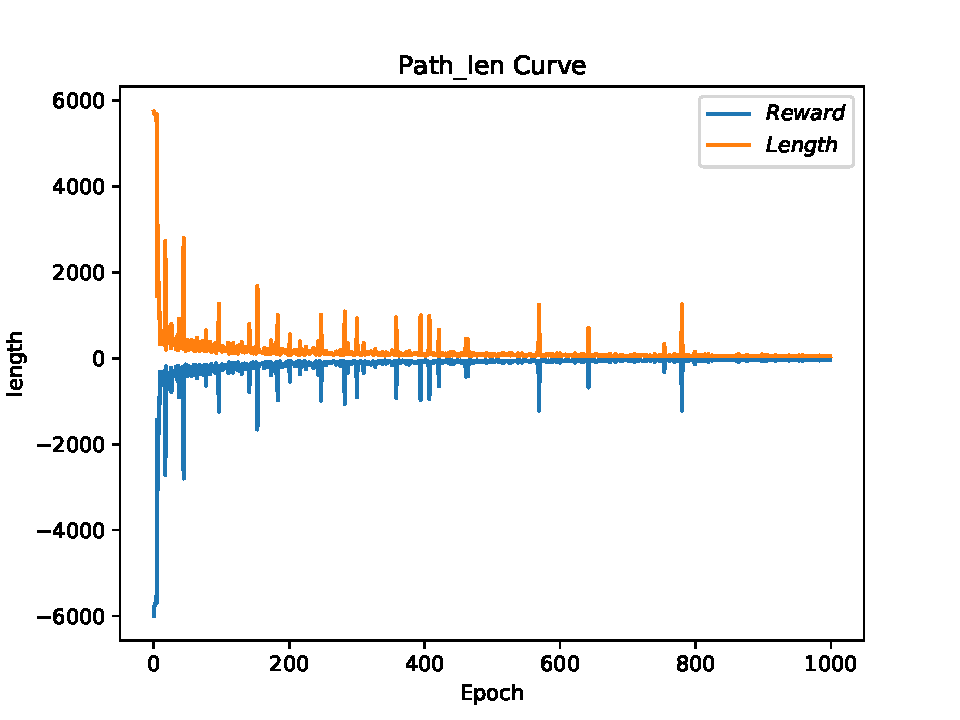
\includegraphics[width=0.5\linewidth]{fig/q_path_length.pdf}
  \caption{\textbf{Q-leaning奖赏路径长度图}}
  \label{fig:4-2}
\end{figure}
路径规划过程中奖赏趋势图,与路径长短随时间变化图
如图~\ref{fig:4-2},可以看到随着迭代轮数的增加,在500epochs左右路径长度和奖励收敛,
之后出现的尖峰是因为是因为执行$\epsilon$贪心策略产生的。因为本文设计
的奖励函数与路径长度相关,所以从图中可以看到其收敛的一致性于对称性。
\subsubsection{SARSA路径规划}
SARSA路径规划效果图
如图~\ref{fig:4-3},可以看到SARSA算法规划出的路径和Q学习规划出的路径长短相差不大。
\begin{figure}[H]
  \centering
  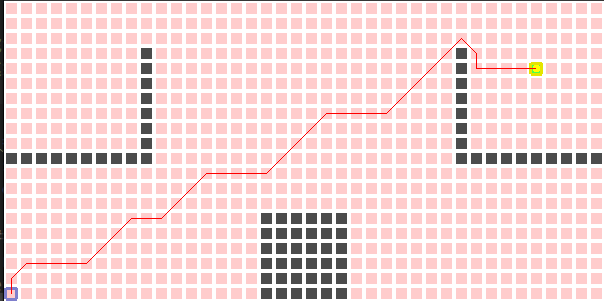
\includegraphics[width=0.8\linewidth]{fig/sarsa1.png}
  \caption{\textbf{SARSA路径规划}}
  \label{fig:4-3}
\end{figure}
路径规划过程中奖赏趋势图,与路径长短随时间变化图如图~\ref{fig:4-4},从图中可以看出,SARSA算法在1000epochs左右收敛,但之后尖峰出现较多,
且幅值较大。对比来看,
Q学习的收敛速度大于SARSA,迭代过程的波动也小于SARSA,所以综合来看,Q学习更实用于路径规划。
\begin{figure}[H]
  \centering
  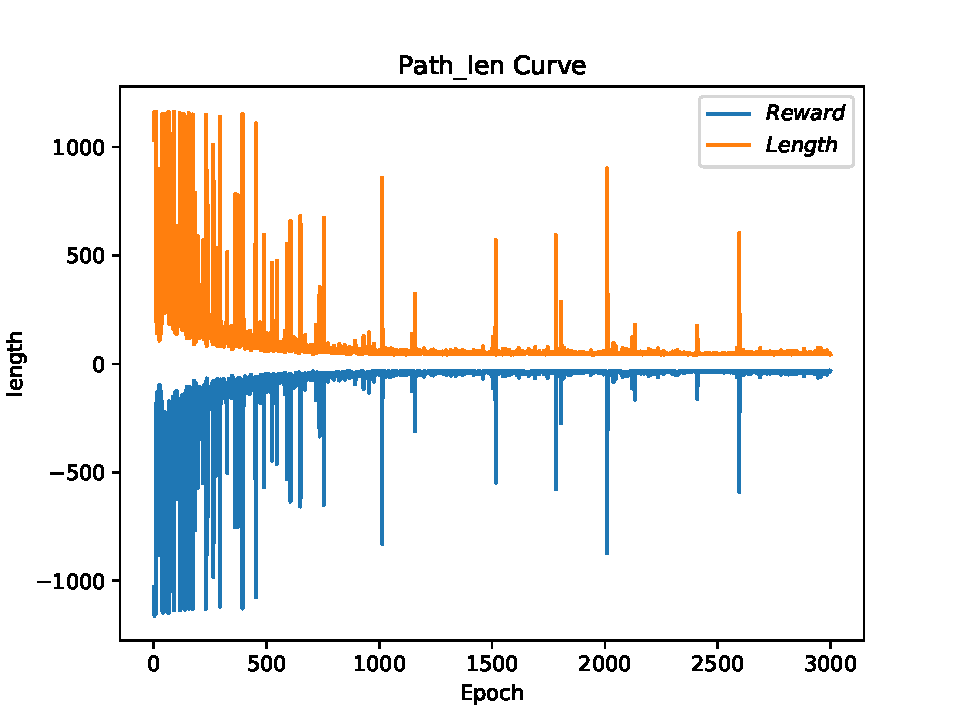
\includegraphics[width=0.8\linewidth]{fig/sarsa_path_length.pdf}
  \caption{\textbf{SARSA奖赏路径长度图}}
  \label{fig:4-4}
\end{figure}

\subsection{DQN车道保持}
\subsubsection{数据预处理}
本文DQN车道保持主要使用了Carla中的语义相机,数据预处理也是主要对语义相机的数据进行处理。首先使用将Carla中的语义标签进行缩减,缩减细节详见本文第二章CARLA中的传感器。
得到缩减后的含有标签数据的Carla语义相机数据后,并使用PIL和Pytorch对图像数据进行尺寸统一化处理,并将其转化成张量送到神经网络中。这样做的目的主要是为了加快模型的训练速度,
并抑制过拟合现象。此外,本文还将Carla中的车辆控制简化为一些离散的控制指令,作为神经网络的输出,即DQN的动作空间。具体为向左向右转向22度,直行。
\subsubsection{车道保持实验结果}
DQN车道保持奖赏图
如图~\ref{fig:4-5}。可以看出随着迭代轮数的增加,奖励值在一定范围内波动最终收敛于0,收敛于0即沿着车道行驶,中间极值的出现是因为车辆运行$\epsilon$贪心策略导致撞到障碍物所以给出了较大的负值奖励,从图中可以看出本文已基本实现了车道保持任务。
\begin{figure}[H]
  \centering
  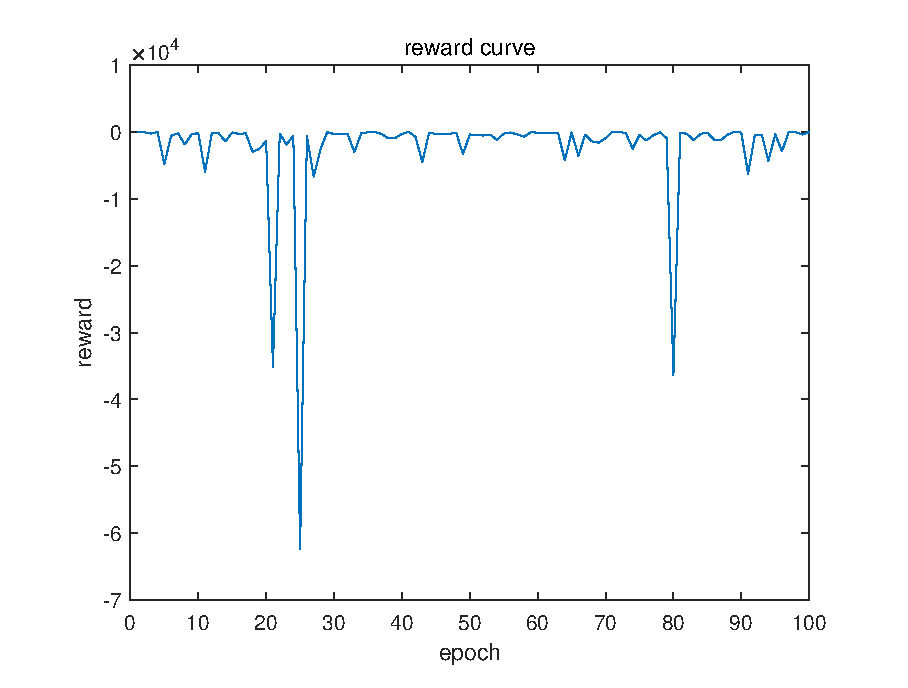
\includegraphics[width=0.5\linewidth]{fig/reward.eps}
  \caption{\textbf{DQN车道保持奖赏图}}
  \label{fig:4-5}
\end{figure}

\subsection{本章小结}
本章主要介绍了强化学习路径规划与深度强化学习车道保持的实验结果,对结果进行了分析。可以看到强化学习路径规划可以很好的体现出奖励函数的要求,基本可以实现本文提出的
“以人为本”的路径规划。针对深度强化学习车道保持,在Carla仿真环境下进行了测试,其结果表明将深度强化学习引入无人驾驶决策模块具有一定可行性。 \sectionend
%% Copyright (C) 2018 Liu Yifan, Zhao Tianyu 
% Permission is granted to copy, distribute and/or modify this document
% under the terms of the GNU Free Documentation License, Version 1.3
% or any later version published by the Free Software Foundation;
% with no Invariant Sections, no FrontCover Texts, and no BackCover Texts.
% A copy of the license is included in the section entitled "GNU
% Free Documentation License".
\section{测试}

 \sectionend


	
	\vspace*{0pt}
	\section*{总结与展望}	
	
	
	\addcontentsline{toc}{section}{总结与展望}
%	本文从最优化理论出发
  
  本文从强化学习路径规划出发,提出可以通过个性化设计奖励函数来达到以人为本的路径规划,对此使用强化学习中的Q学习算法和SARSA算法进行了验证,实验结果表明
Q学习算法可以较好的满足奖励函数的要求。虽然如此,但如何设计奖励函数来体现用户的需求也是一大难题,后续可以通过使用深度逆强化学习反向解析用户习惯,得到用户
的个性化奖励函数。
针对无人驾驶决策领域的挑战,本文提出使用深度强化学习中的DQN算法来代替传统的无人驾驶决策模块,实现车道保持
任务,对此想法在Carla仿真环境中进行验证,可以看到DQN车道保持算法基本可以实现车道保持,但也具有一定缺陷。由于动作空间较少的原因,车道保持的过程会出现一定的左右摇摆现象,为什么不选取多动作空间是因为多动作空间神经网络的训练过于耗时,所以本文只选取了三个值的动作空间加快训练,且三动作空间下DQN的车道保持效果也可以令人接受,动作空间的选取较好的折中了计算资源和实验效果。训练过程中由于$\epsilon$贪心策略的存在车辆有时会去往错误的地方,后续可以加入规则进行限制。
综上可以看出
深度强化学习在无人驾驶决策领域是可以大有所为的,此外在后续神经网络的训练过程中也可以加入专家样本来指导神经网络,加快神经网络的收敛,提升神经网络的性能。
   

	
	
	
	\sectionend
	\addcontentsline{toc}{section}{参\ 考\ 文\ 献}
	\begin{small}	
		\setlength{\bibsep}{0ex}
		\vspace*{0pt}
		\bibliographystyle{thuthesis-bachelor}
		\bibliography{refs}
	\end{small}
		
	

	\sectionend	
	
	\vspace*{0pt}
	\section*{\centerline{致\hspace*{3em}谢}}
	\addcontentsline{toc}{section}{致\hspace*{1em}谢}
	%\zihao{-4}{
	感谢大连海事大学四年的培养,感谢本科阶段所有的老师,他们在我获取知识的途中给予了我巨大的帮助。在所有老师中特别需要感谢的
为本科指导教师陈余庆老师,他给了我论文许多建议,使我受益匪浅。感谢答辩的评审老师,感谢你们在百忙之中,抽出时间检查我的成果。
本科论文就像是一个对本科生涯的总结,它的完成当然也离不开我在本科阶段遇到的朋友,老师,以及一直在背后支持我的家人。此外还要感谢
清华大学和大连海事大学Latex模板以及开源社区和问答社区的所有开发者,他们的工作和回答,使我免去了许多重复的工作。

最后,感谢所有评审老师和专家,感谢你们抽出宝贵的时间审查我的论文,希望你们对本篇论文提出宝贵的意见。
	
%	\sectionend	
	
%	\vspace*{0pt}
%	\section*{\centerline{附\hspace*{3em}录}}
%	\addcontentsline{toc}{section}{附\hspace*{1em}录}

%\begin{figure}[htbp!]
% 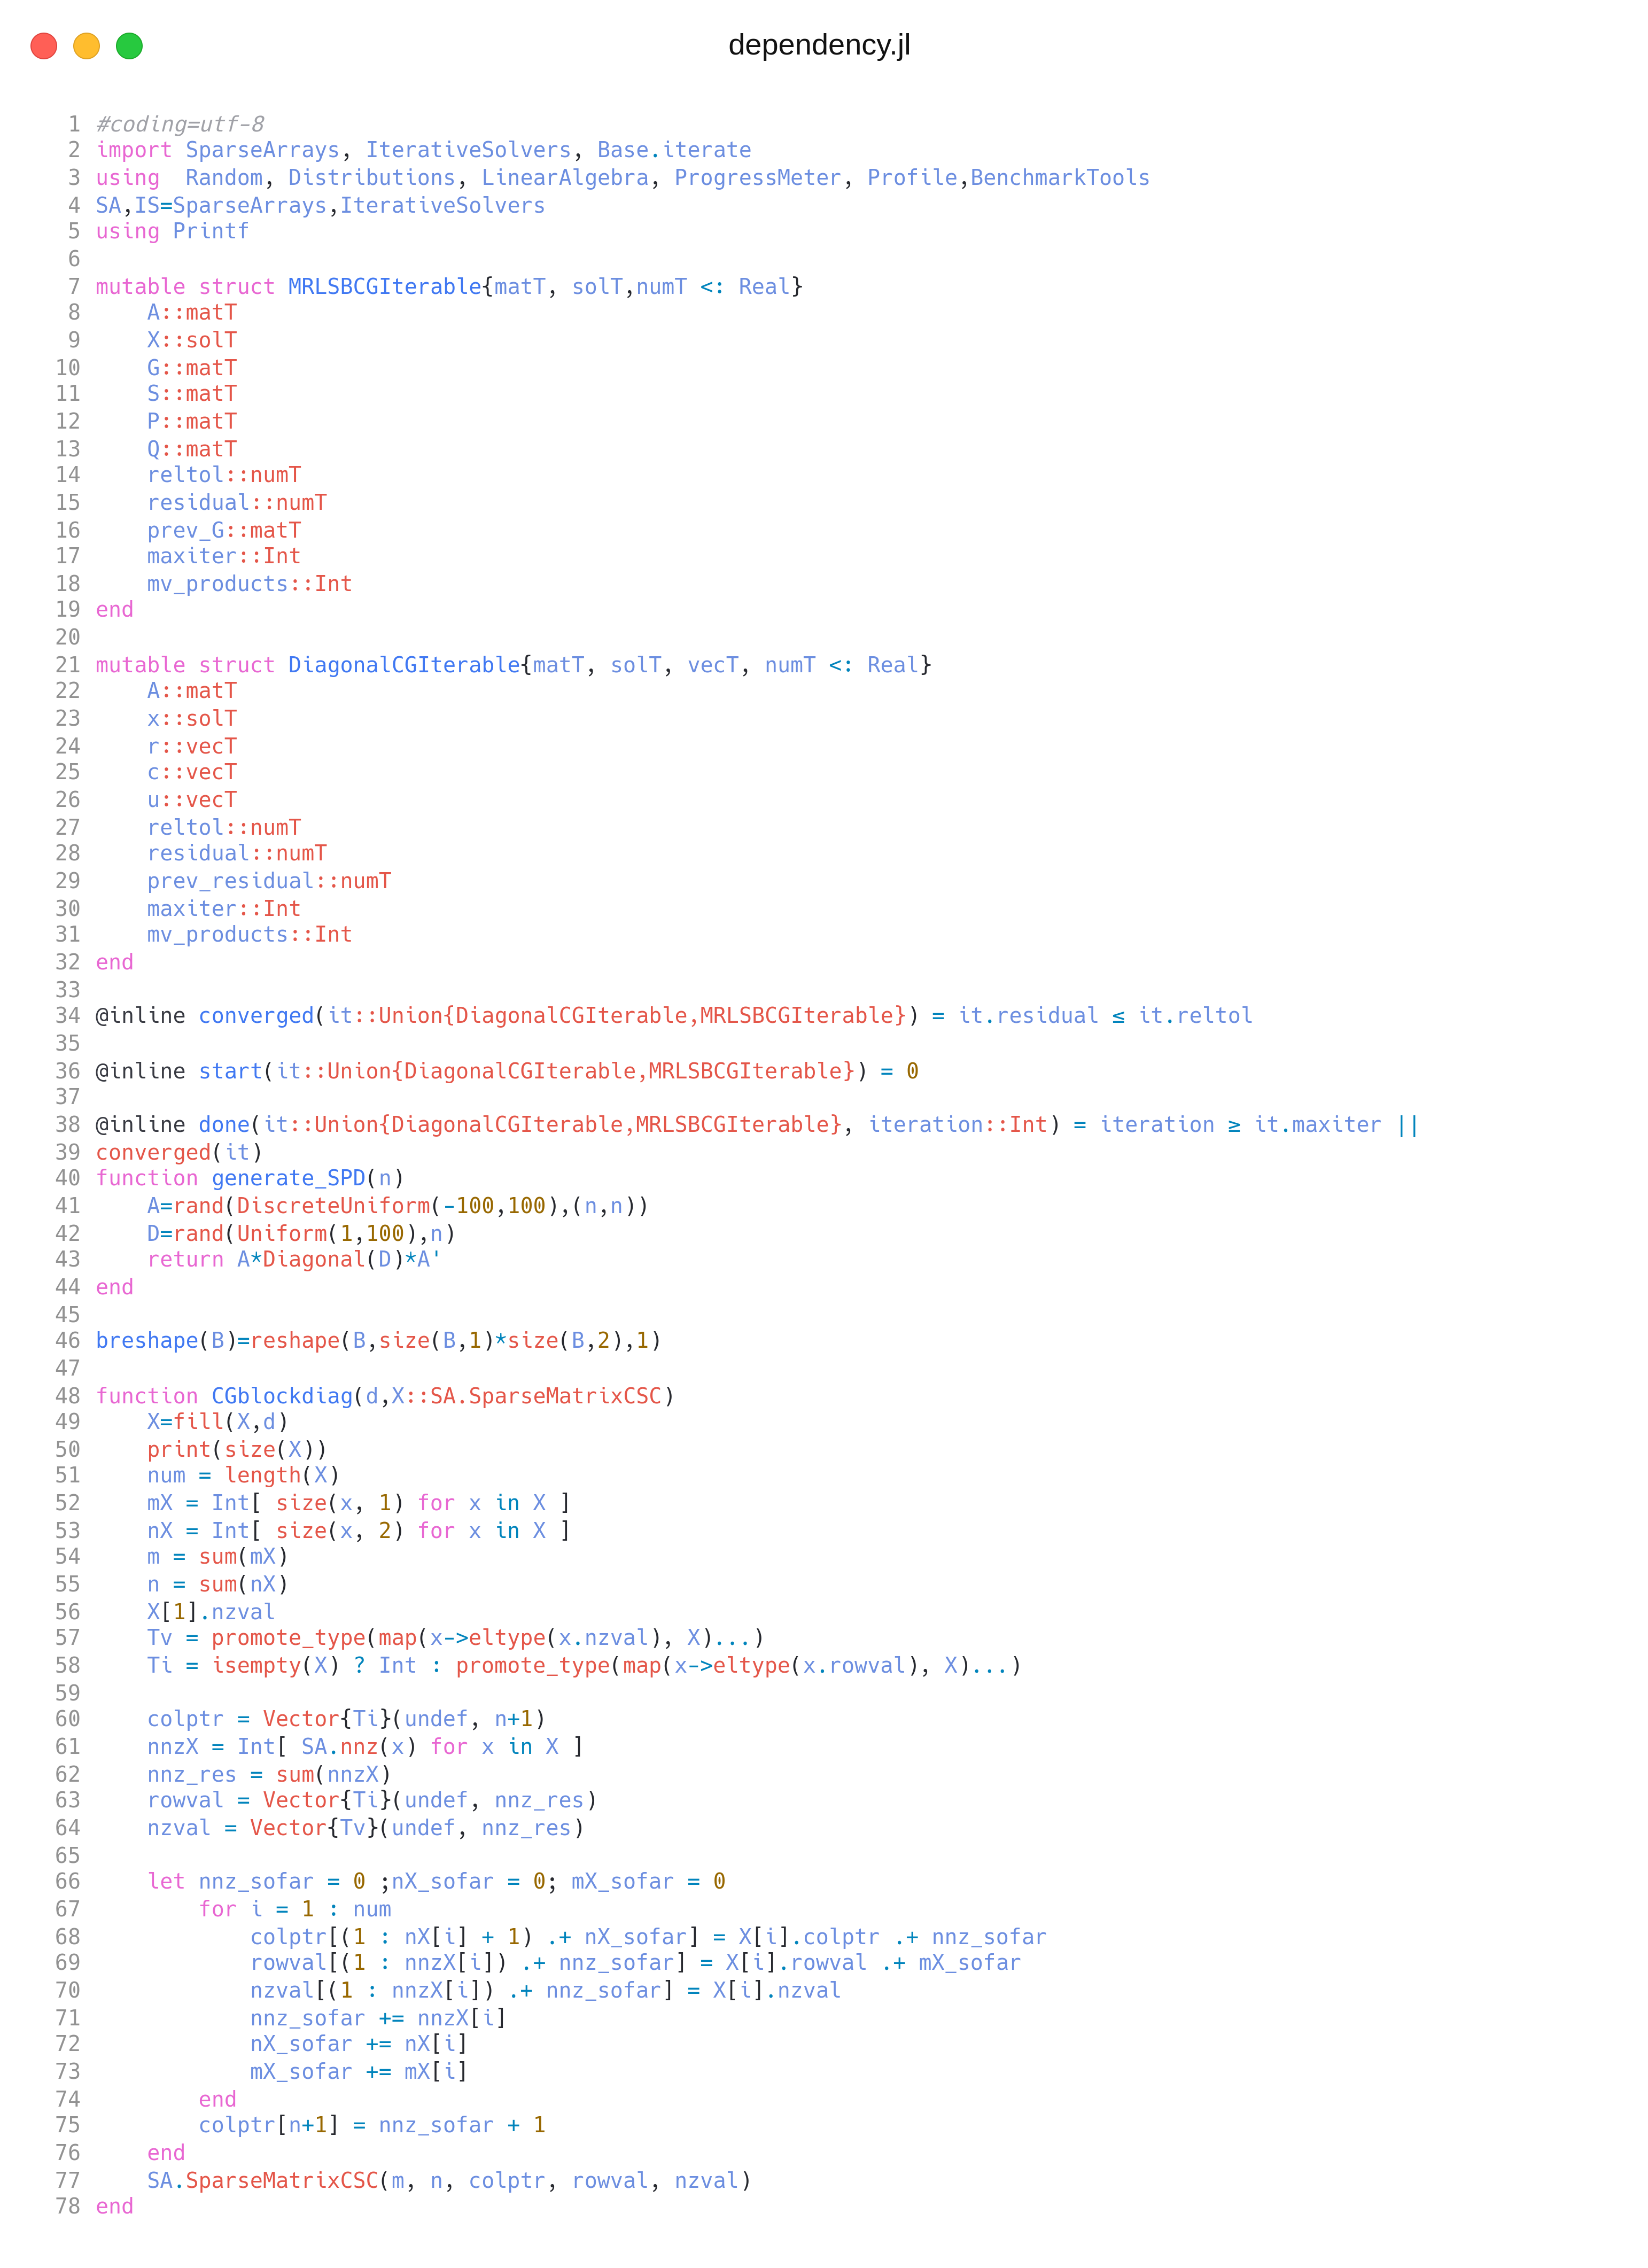
\includegraphics[height=0.9\textheight]{code/dependency.png}
% \end{figure}	    

\end {document}